%!TEX root = Memoria_TFM.tex
\begin{small}
\emph{In this chapter, is explained the programming language used, the databases that are going to be trained and tested, the classifiers with which test samples are going to be tested and metrics used to compare results.}
\end{small}

%!TEX root = Memoria_TFM.tex
\section{Programming language and frameworks}
The  programming language which has been used to develop the thesis is \textit{Python}. \textit{Python} is an object-oriented language and very used nowadays. The version used is the 2.7.\\

\textit{Python} libraries have been used to help to implement the code. The main framework used is \textit{Theano}. \textit{Theano} has been used to build the convolutional neural network and its training procedure because of the possibility that offers of working with symbolic variables, mathematical expressions and multidimensional arrays. \textit{Theano} documentation could be found in \url{http://deeplearning.net/software/theano/}.\\

\textit{Scikit-learn} is another \textit{Python} library which has been used as the basis of building the classifiers and some of the metrics. Its documentation it is available in the following url \url{https://docs.scipy.org/doc/numpy/}.\\

Others libraries such as \textit{NumPy} or \textit{Matplotlib} have been needed. \textit{NumPy} is a library that allows users to works with multidimensional arrays or random simulations among others qualities. The documentation of this framework is available in \url{https://docs.scipy.org/doc/numpy/}. \textit{Matplotlib} has been utilized as graphic tool to plot figures.

%!TEX root = Memoria_TFM.tex
\section{Databases}
In this section the databases that are used along the thesis are described in this section.\\

One database has utilized to learn \textit{Theano} and three face databases has been used in order to detect anti-spoofing. The face anti-spoofing databases have been generated with face anti-spoofing finality and has been used previously with the same purpose.\\

All the databases are formed by three subsets whose samples are not repeated among subsets:
\begin{description}[itemsep=2pt,topsep=8pt,parsep=0pt,partopsep=20pt]
\item[Training subset:] is used to train the network during epochs.
\item[Validation subset:] is used to check the performance of the network while is training. The validation subset is usually used when hyper-parameters are calculated.
\item[Test subset:] is used just at the end of the training process. The best model is chosen with regard to the best validation error. This subset should not be used until the network architecture and classifiers parameters are selected.
\end{description}

\subsection{MNIST digit database}\label{subsec:MNIST}
MNIST digit database is a image database of human written digits. This database is frequently used to learn machine learning techniques. Because of that, the database has been used, in this thesis, for learning Theano and convolutional neural networks. In addition, this database has been used in a implemented convolutional neural network (LeNet).\\
\begin{figure}[htb]
\centering
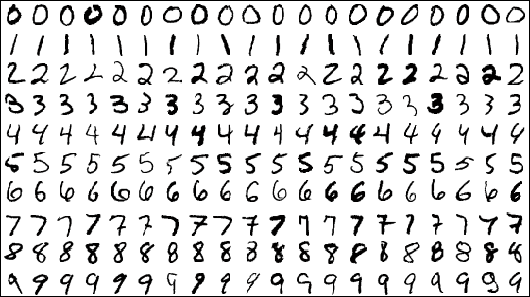
\includegraphics[width=0.6\textwidth]{images_databases/mnistExamples.png}
\caption{MNIST digit images database. Image obtained from \cite{MNISTimage}} \label{fig:MNIST_digits}
\end{figure}
Some examples of the digit image MNIST database could be seen in \ref{fig:MNIST_digits}, image obtained from \cite{MNISTimage} and the characteristics of this database are the following ones:
\begin{itemize}[itemsep=2pt,topsep=8pt,parsep=0pt,partopsep=20pt]
 \item There are 70.000 number of unique samples.
 \item Despite of the original size of the database is 32x32 pixels, the samples of this downloaded database are 28x28 pixels in gray scale, that is 784 features per image.
 \item 10 classes could be differentiated, one per digit.
\item The samples are directly separated into train, test and validate subset.
\end{itemize}

\subsection{FRAV dataset}
FRAV database is an anti-spoofing face database built in the  \textit{FRAV} research group of the \textit{URJC University} and which is part of the Automated Border Control Gates for Europe project \cite{ABC4EU}.\\

FRAV database is formed by genuine users and spoofing attacks. Moreover, this database is formed by RGB images and NIR images, almost each RGB sample has been captured with infrared camera too.\\

Both databases are composed by genuine users samples and four distinctive attacks: printed photo, 2D mask, 2D mask with eyes cropped and real user image displayed in a tablet device.\\

\begin{itemize}[itemsep=2pt,topsep=8pt,parsep=0pt,partopsep=20pt]
 \item Original images of people represented in figure \ref{frav_im1-4} and figure \ref{frav_im2-5} for RBG images and figure \ref{frav_im3-5} for NIR image.
 \item Images of people printed (attack) represented in figure \ref{frav_im1-1} and figure \ref{frav_im2-1} for RBG images and figure \ref{frav_im3-1} for NIR image.
 \item Images of people with a mask (attack)represented in figure \ref{frav_im1-2}and figure \ref{frav_im2-2}for RBG images and figure \ref{frav_im3-2} for NIR image.
 \item Images of people with a mask with the eyes cropped (attack)represented in figure \ref{frav_im1-3} and figure \ref{frav_im2-3} for RBG images and figure \ref{frav_im3-3} for NIR image.
 \item Images of people in a tablet (attack)represented in figure \ref{frav_im1-4} and figure \ref{frav_im2-4} for RBG images and figure \ref{frav_im3-4} for NIR image.\\
 \end{itemize}

The characteristics of this database are described:
\begin{itemize}[itemsep=2pt,topsep=8pt,parsep=0pt,partopsep=20pt]
\item There are 939 people in each RGB class and 195 in each NIR class.
\item There are 2 or 5 classes: genuine class and four attacks that could be put in the same class or not.
\item Each user has a genuine image and four attacks.
\item There is one image per person.
\item Each image has its own shape.
\item The faces are centered in the image.
\item RGB images has been obtained with a professional visible light camera and NIR images with a Near infrared camera.
\item RGB images are in RGB space and NIR images are in gray-scale space.
\end{itemize}

\subsubsection{FRAV RGB database}
A representation of RGB database is shown in figure \ref{fig:RGB-frav1}, where genuine user (e) and attacks (a-d) from the same user are exposed.\\

\begin{figure}[htb]
\centering
\subfigure[printed image attack]{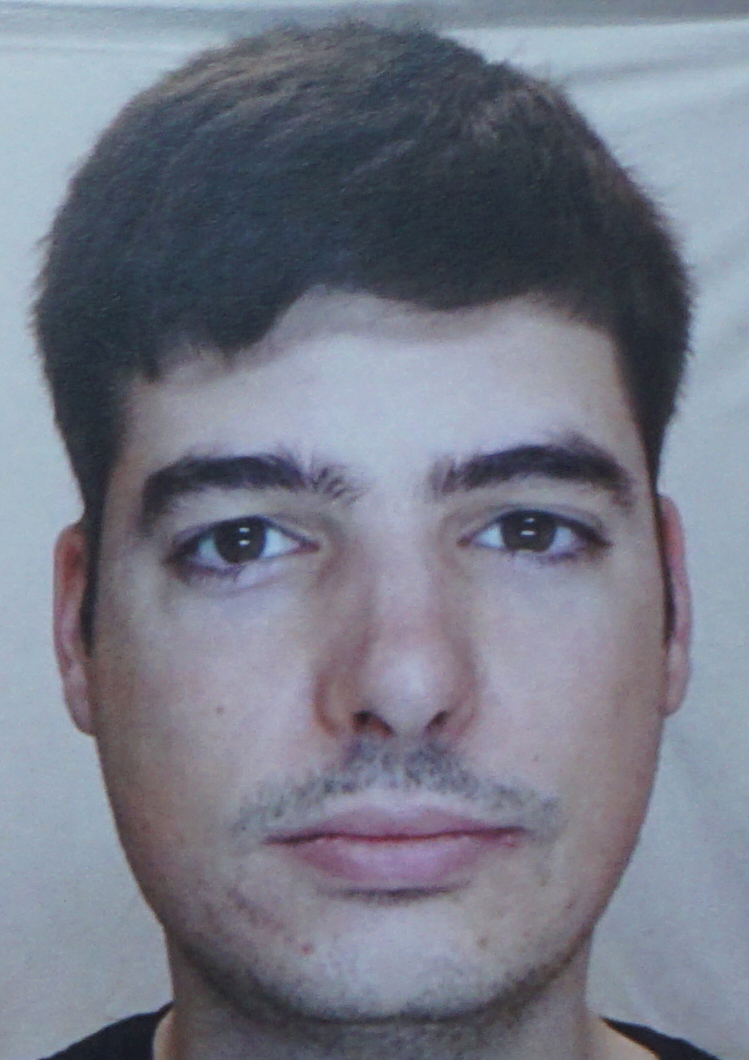
\includegraphics[width=0.18\textwidth]{images_databases/fravrgb/at1-0.JPG} \label{frav_im1-1} }
\subfigure[mask attack]{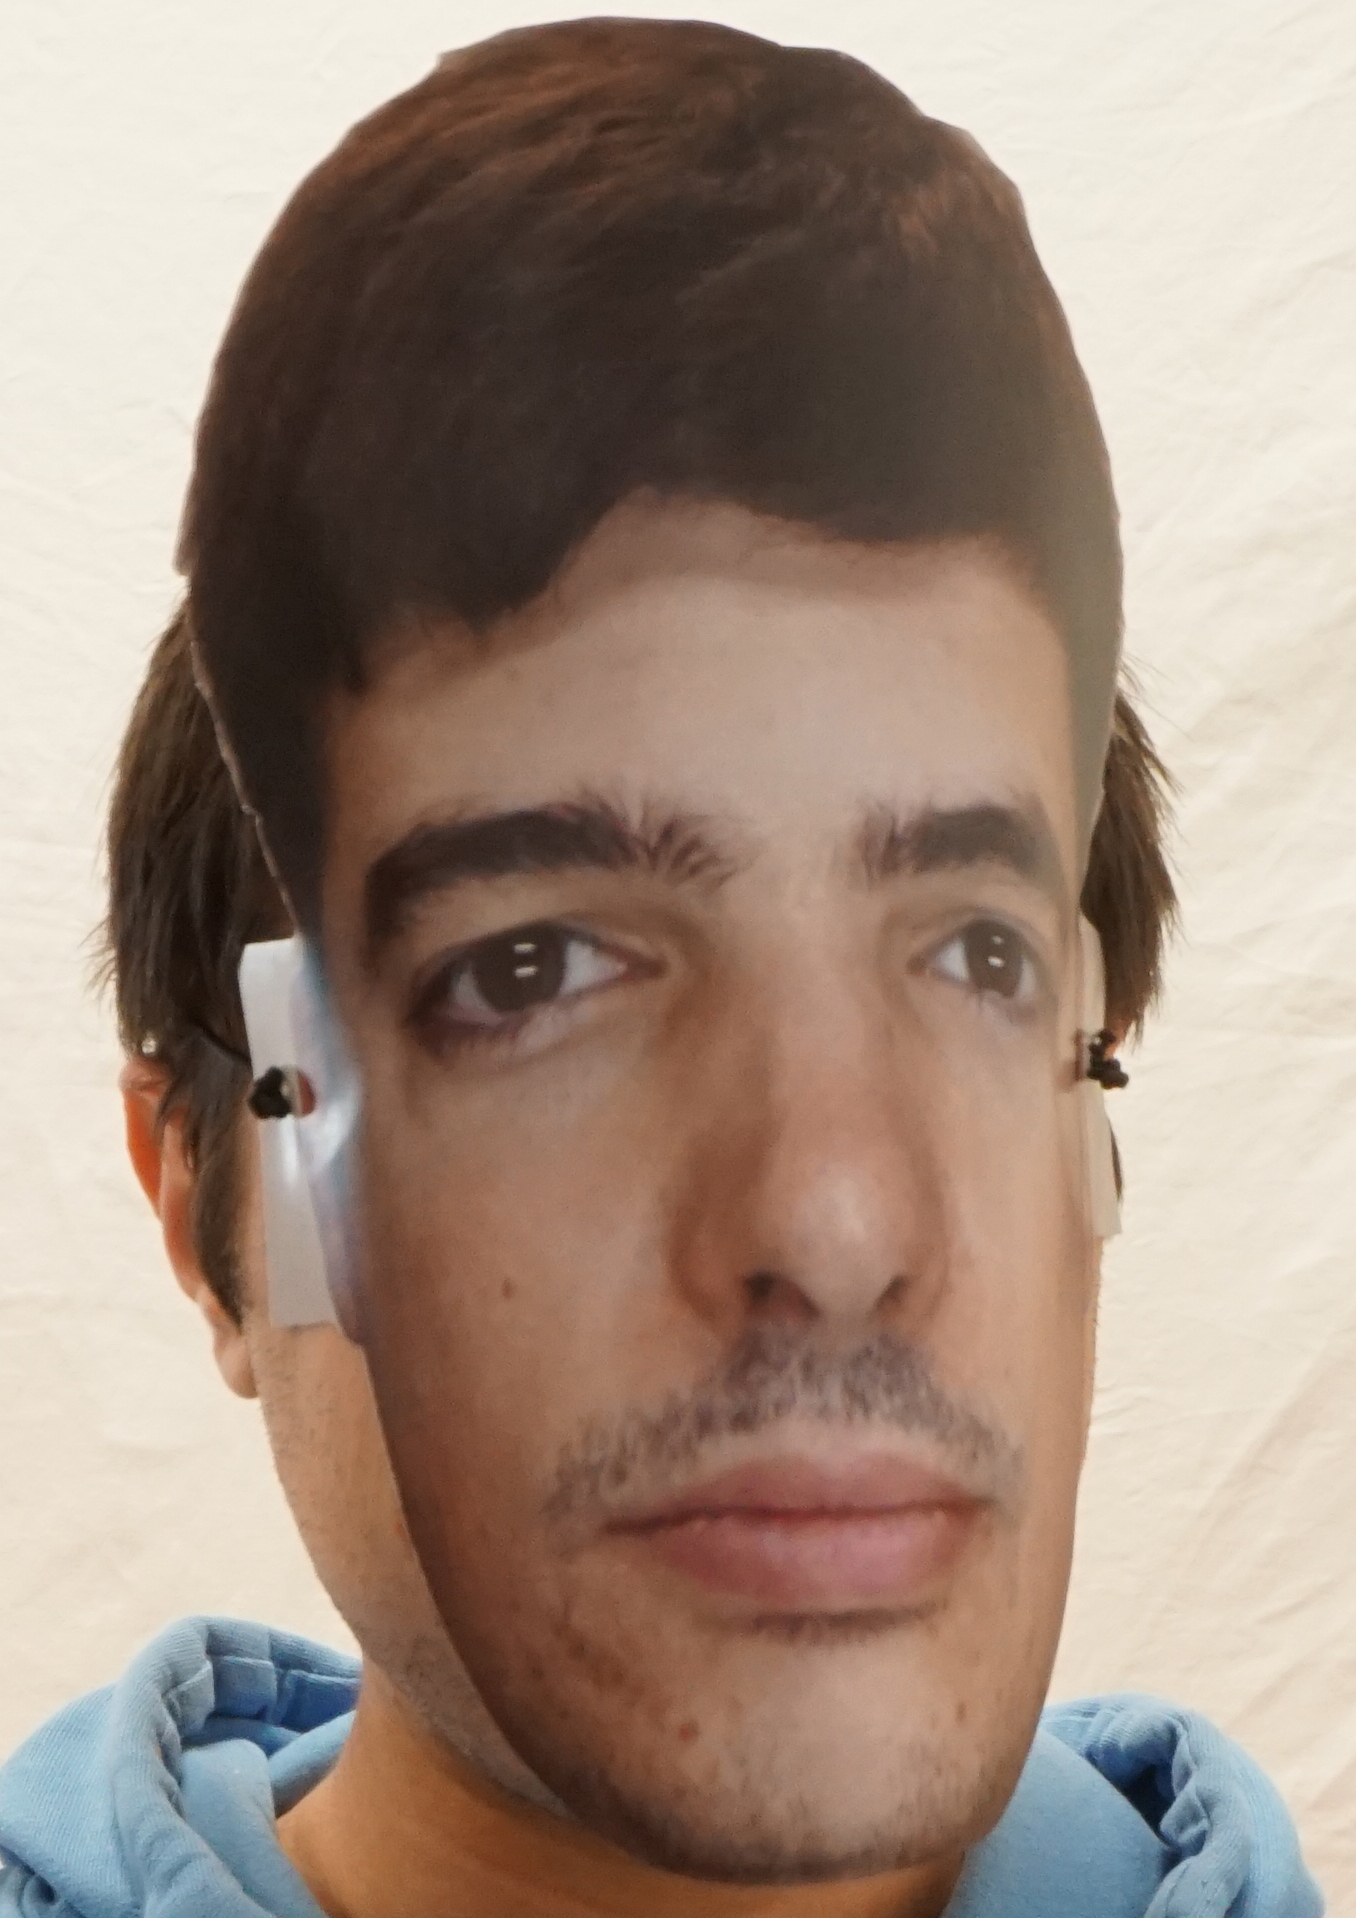
\includegraphics[width=0.18\textwidth]{images_databases/fravrgb/at2-0.JPG} \label{frav_im1-2}}
\subfigure[eye mask attack]{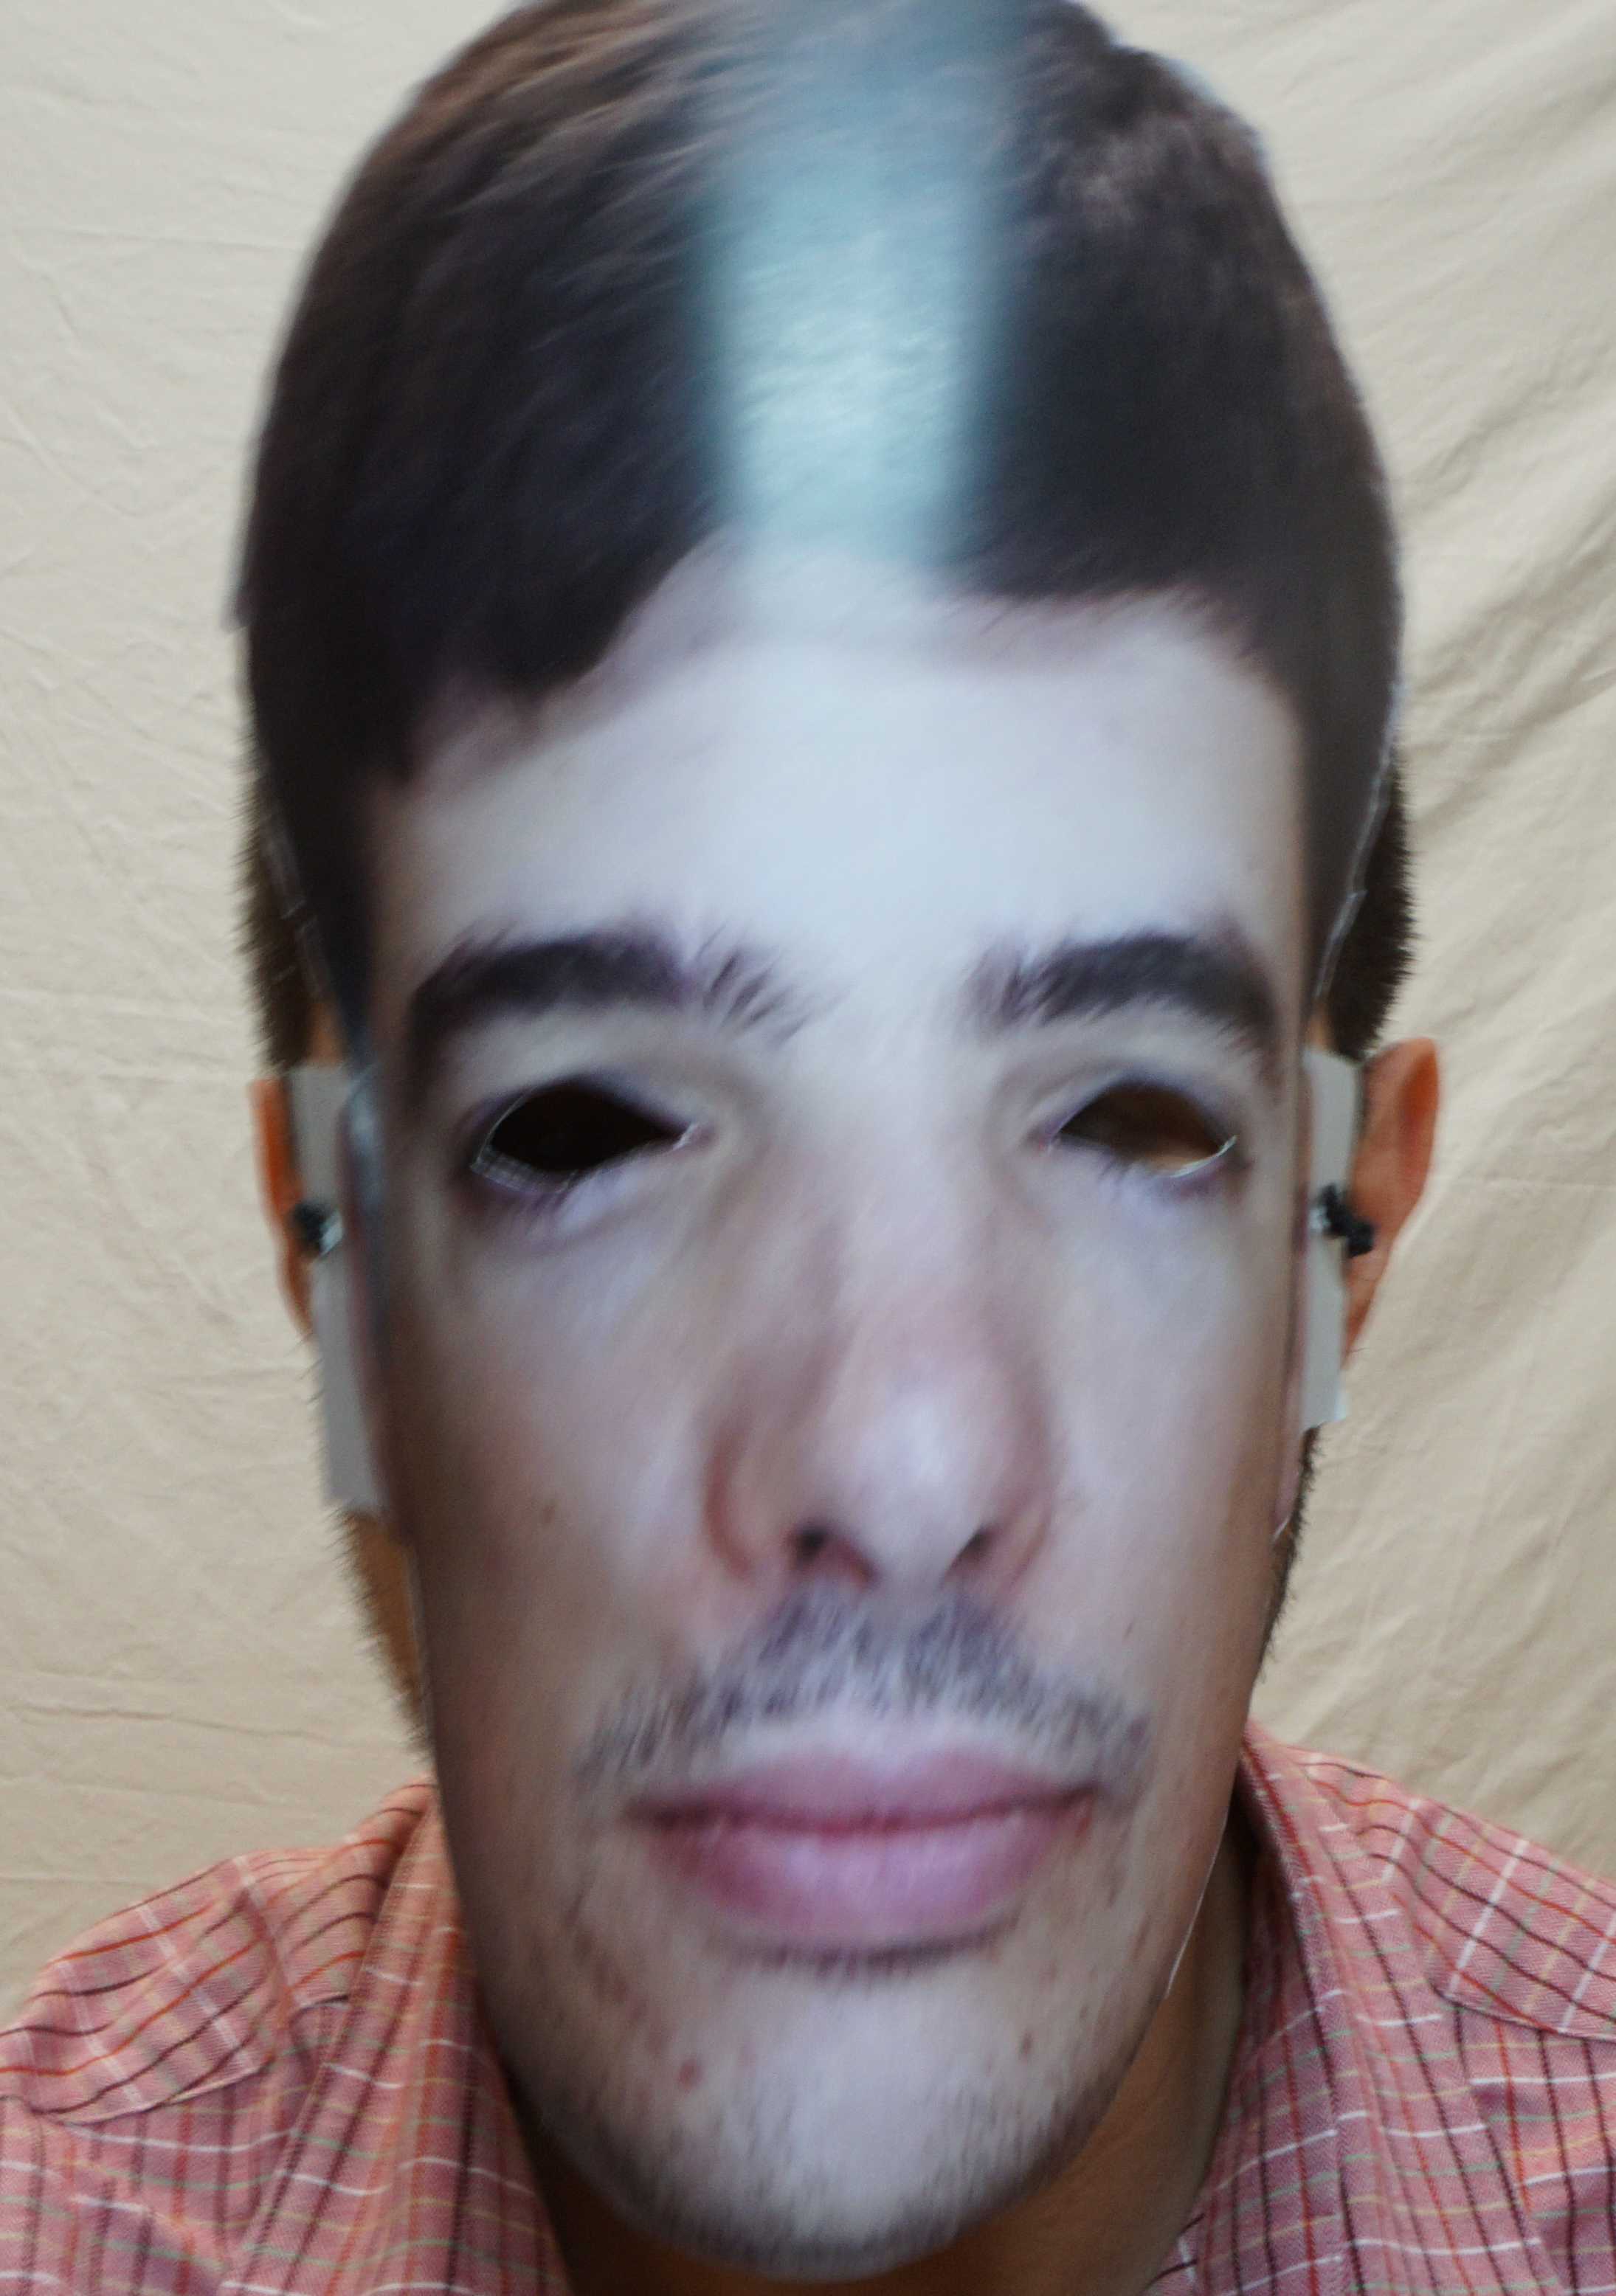
\includegraphics[width=0.18\textwidth]{images_databases/fravrgb/at3-0.JPG} \label{frav_im1-3}}
\subfigure[tablet attack]{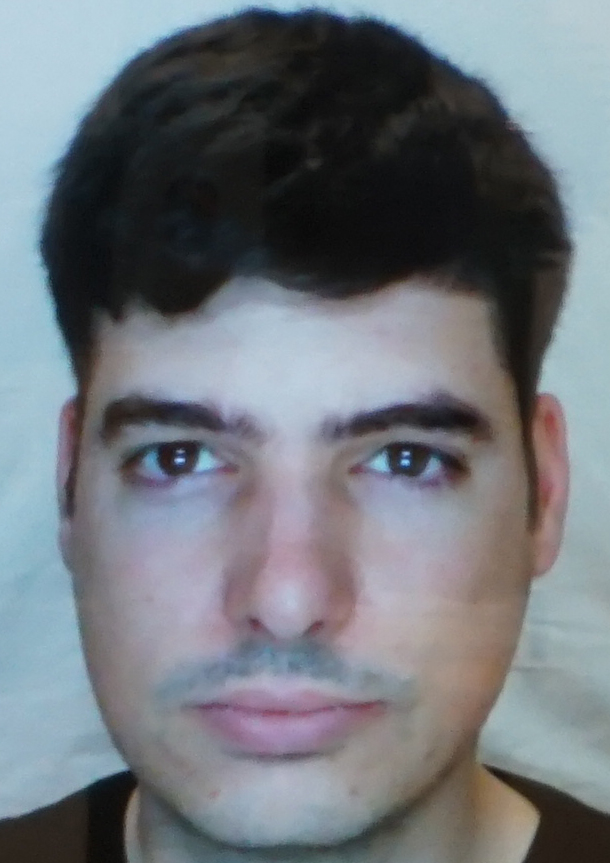
\includegraphics[width=0.18\textwidth]{images_databases/fravrgb/at4-0.JPG} \label{frav_im1-4}}
\subfigure[real user]{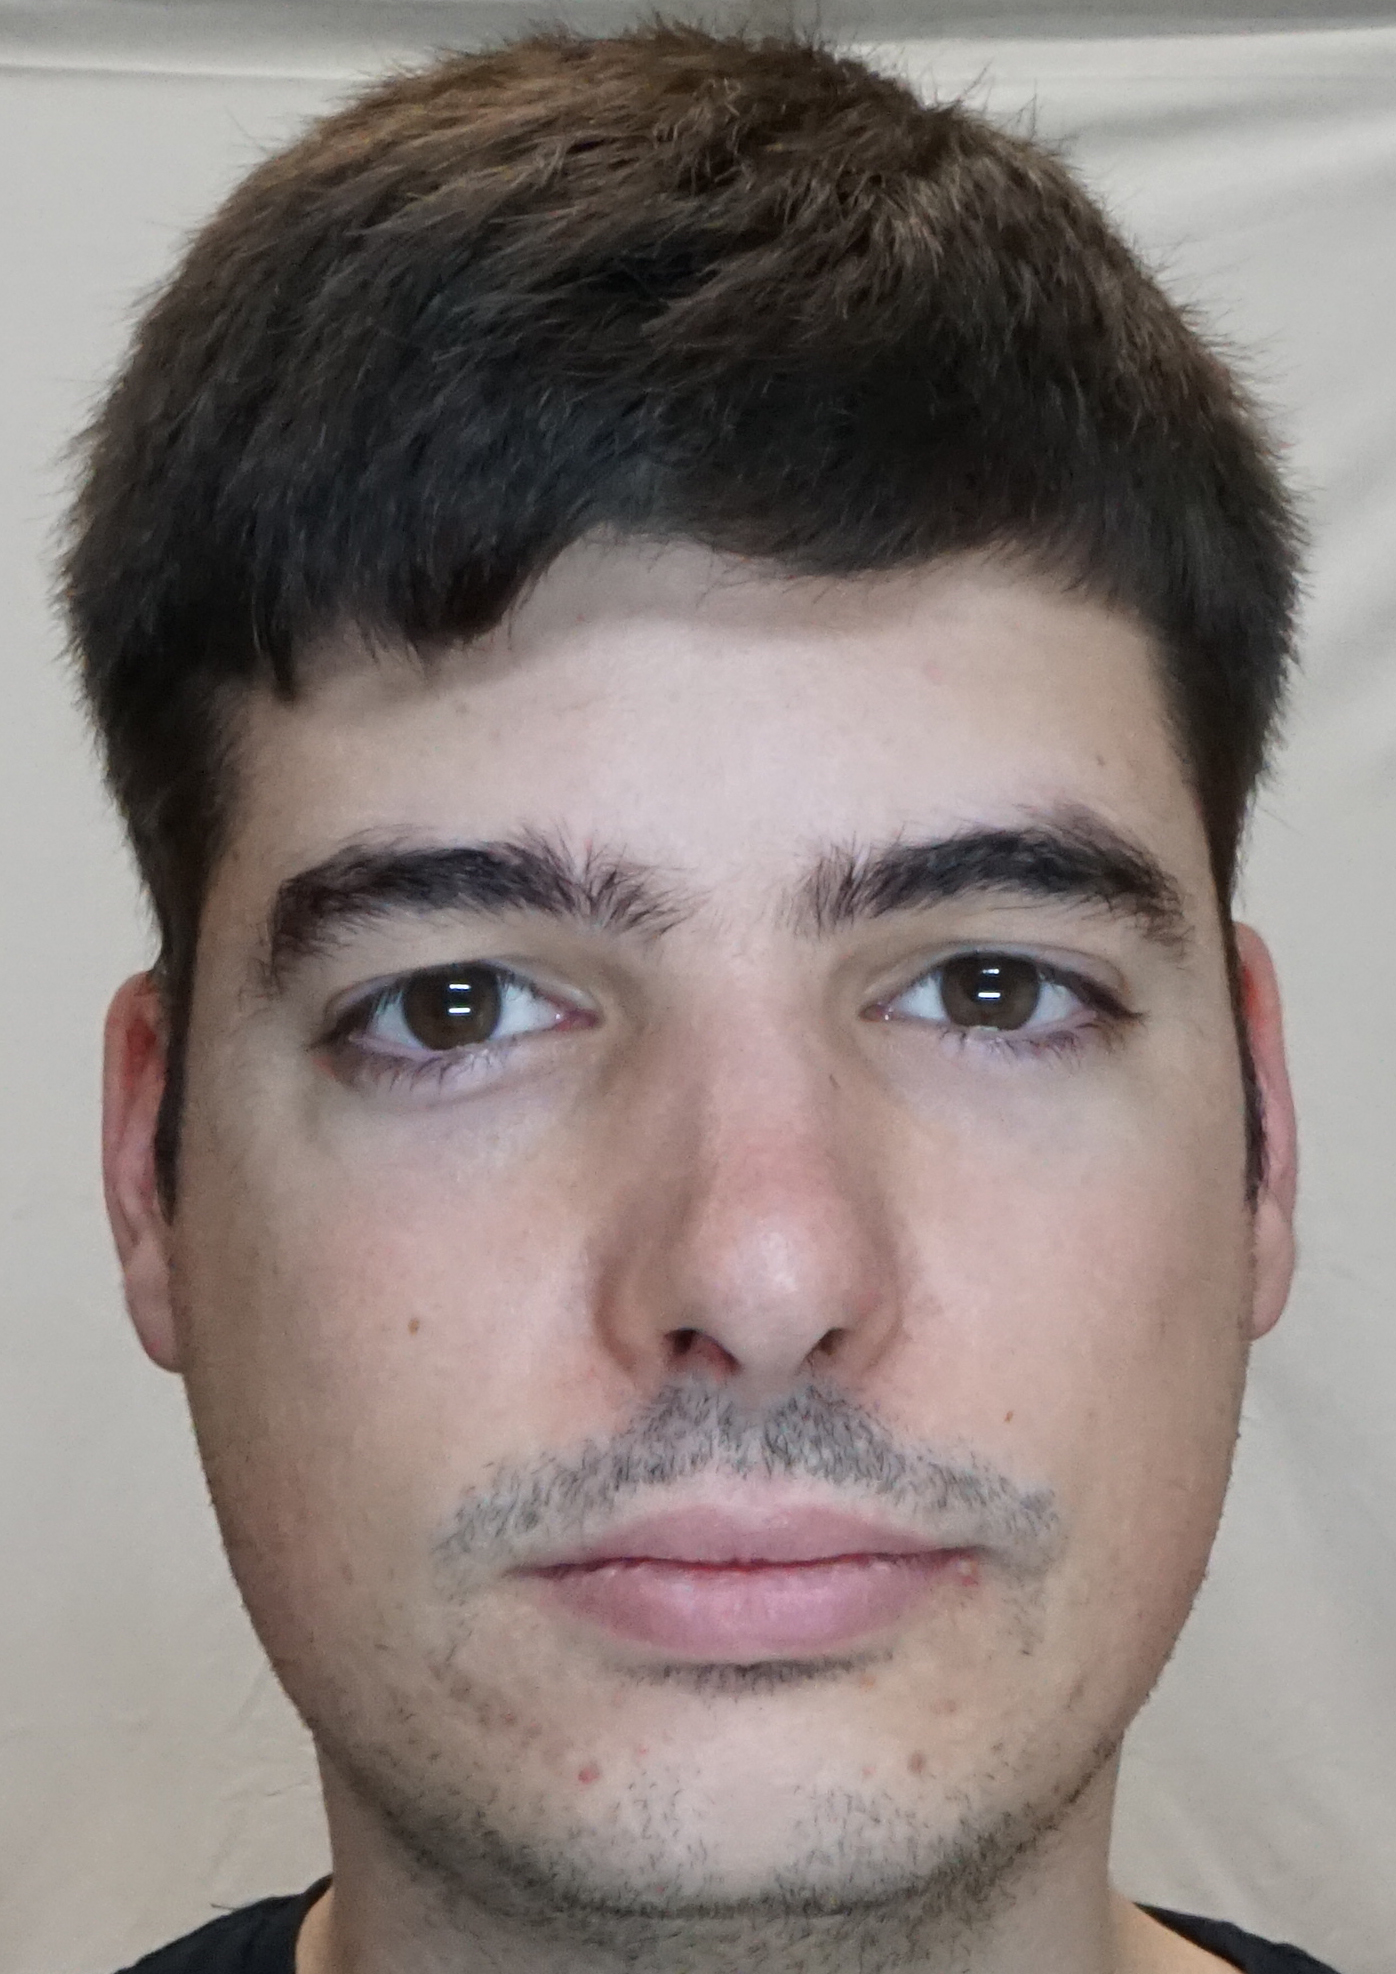
\includegraphics[width=0.18\textwidth]{images_databases/fravrgb/real0.JPG} \label{frav_im1-5}}
\caption{Four attacks and real user from RGB FRAV database } \label{fig:RGB-frav1}
\end{figure}

\subsubsection{FRAV RGB+NIR database}
This database is smaller that RGB database because not all users have its corresponding NIR image. A representation of RGB database is presented in figure \ref{fig:RGB-frav2}, where each RGB image has its corresponding NIR image.\\

\begin{figure}[htb]
\centering
\subfigure[printed RGB image attack]{ 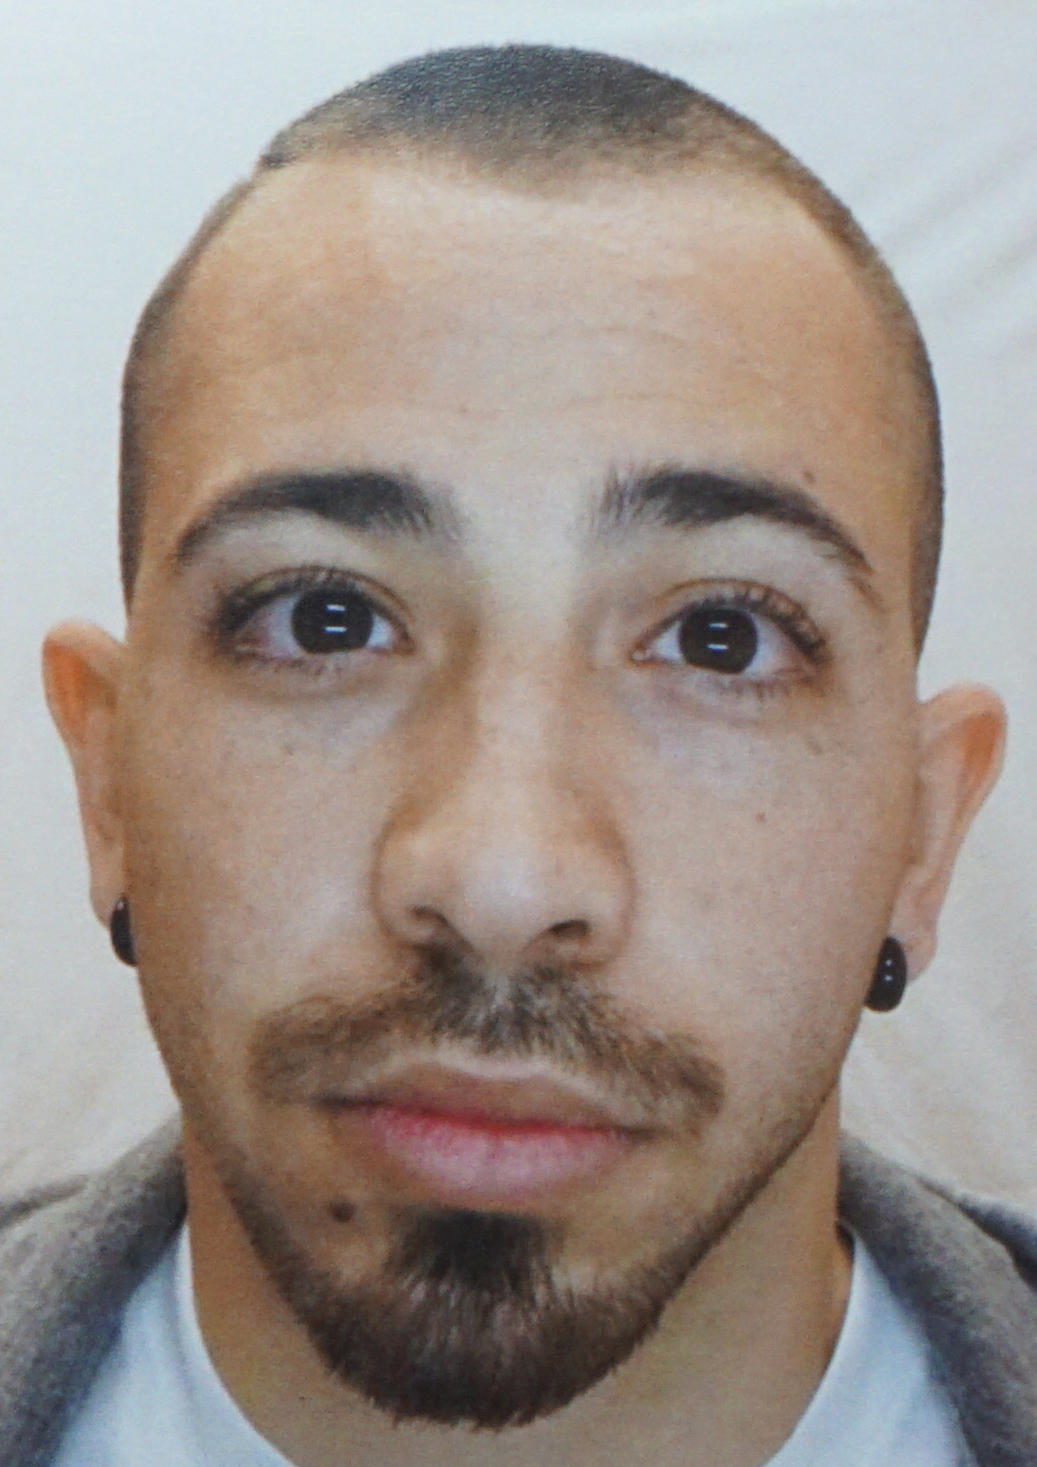
\includegraphics[width=0.18\textwidth]{images_databases/fravrgb/at1-1.JPG} \label{frav_im2-1} }
\subfigure[mask attack RGB]{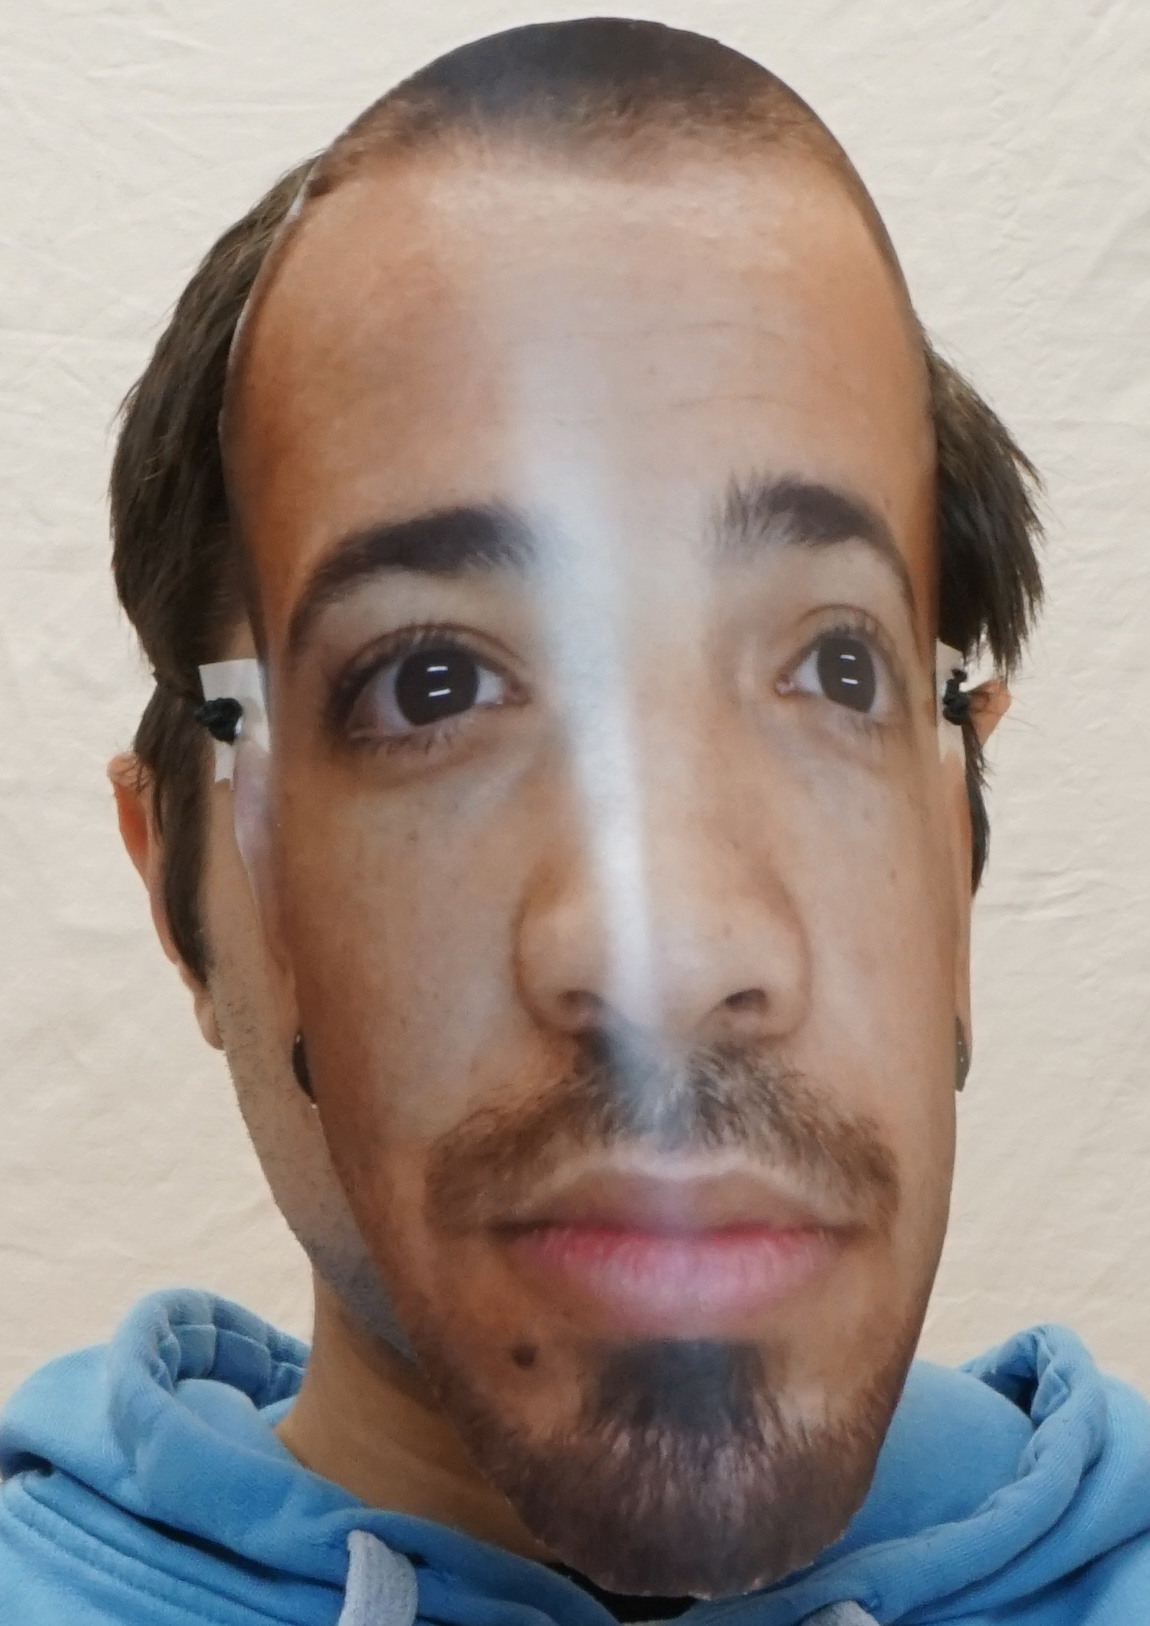
\includegraphics[width=0.18\textwidth]{images_databases/fravrgb/at2-1.JPG} \label{frav_im2-2}}
\subfigure[eye mask attack RGB]{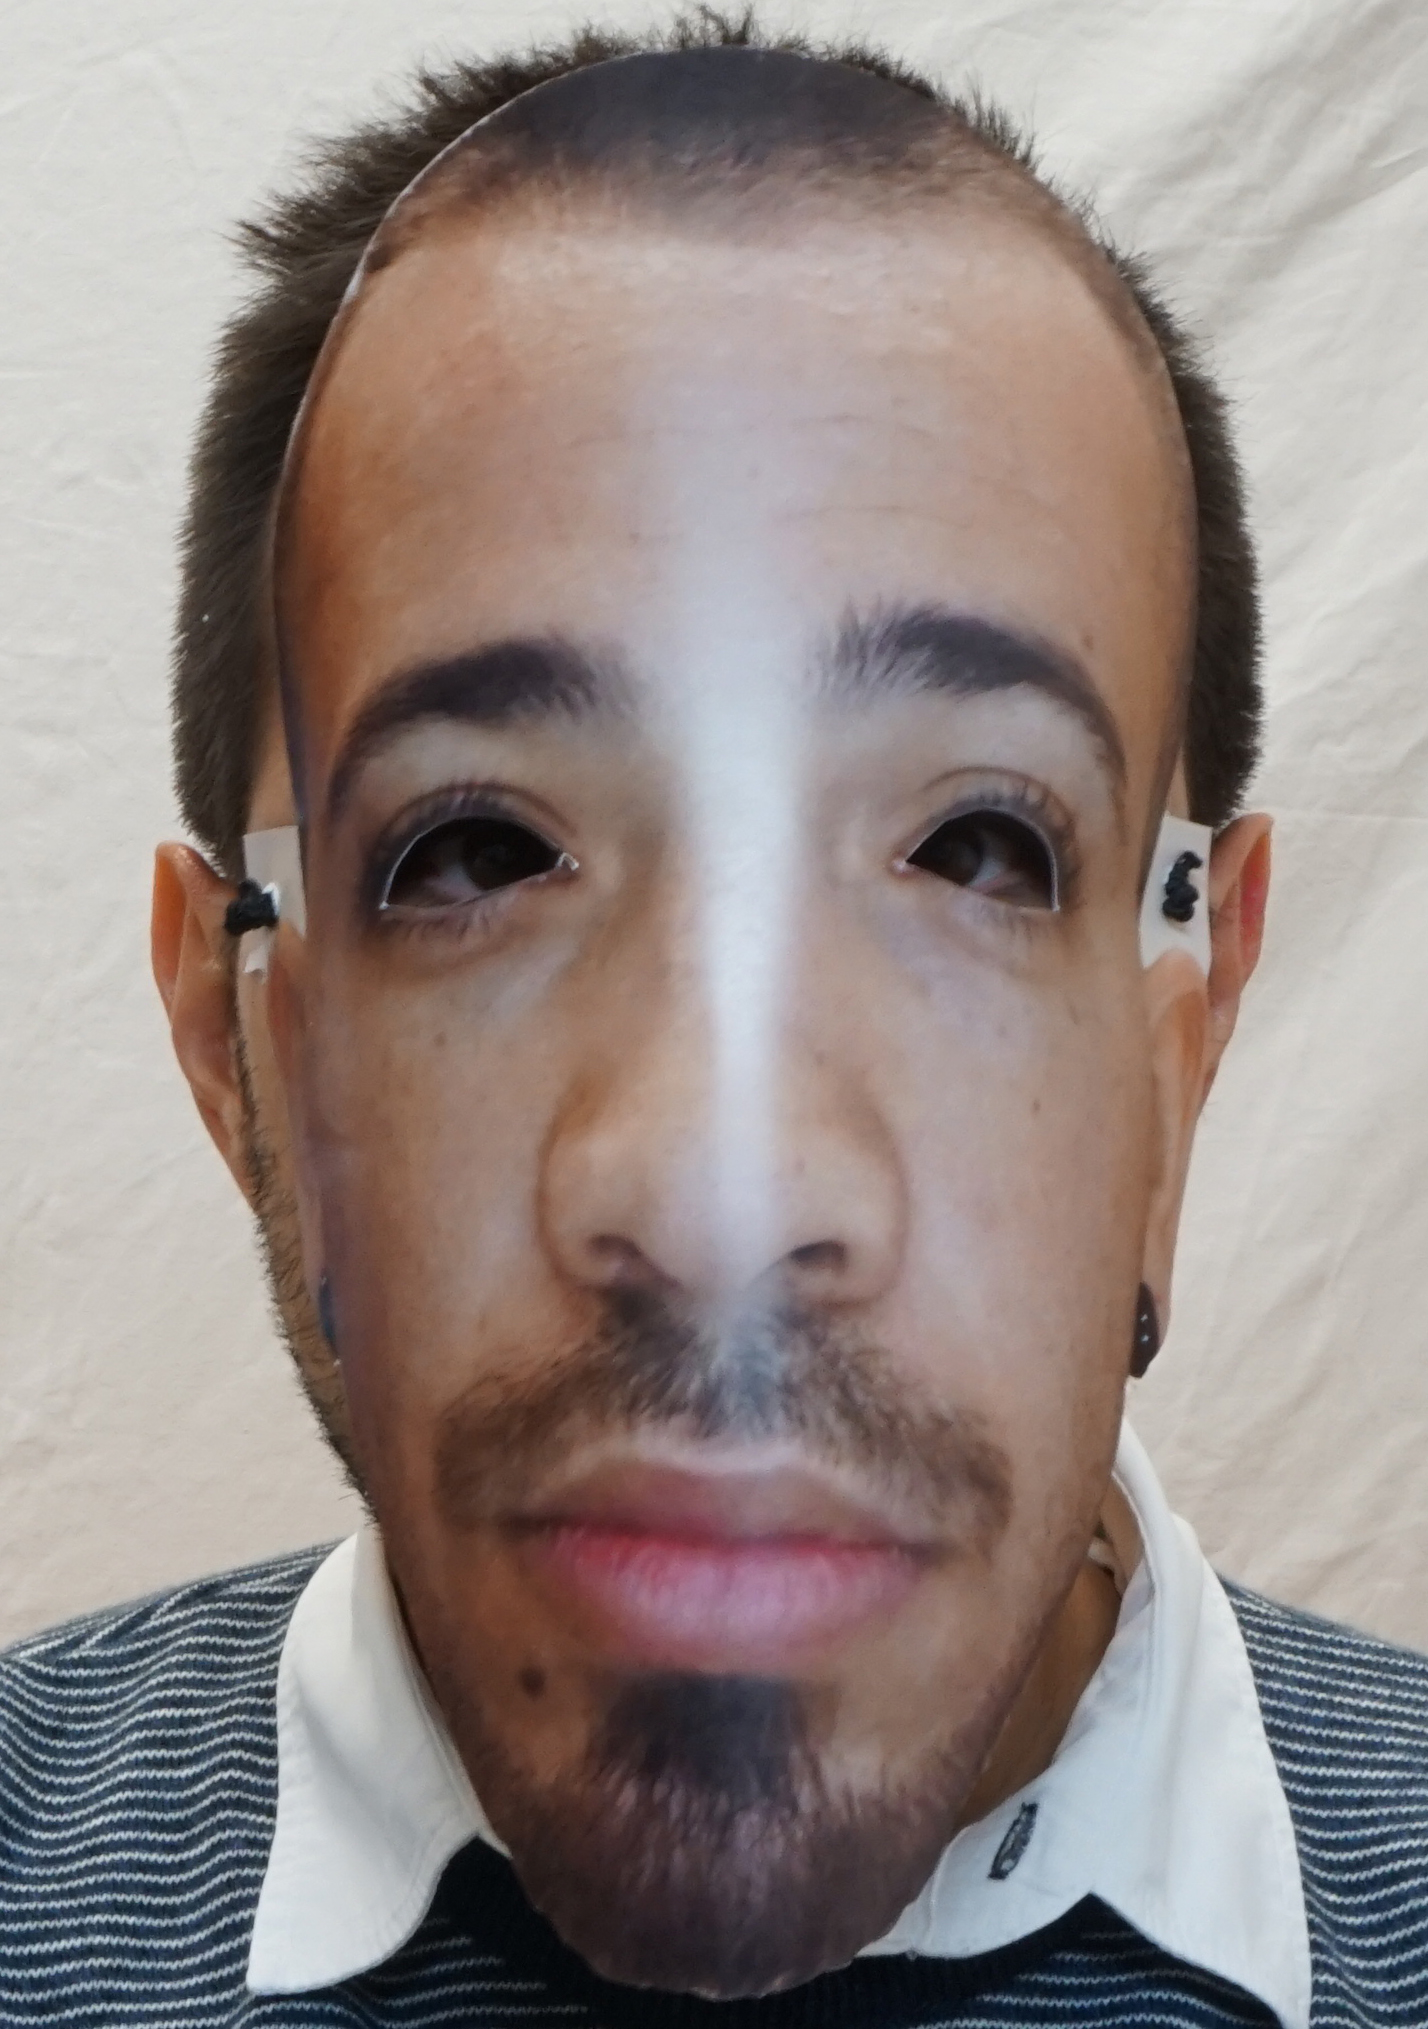
\includegraphics[width=0.18\textwidth]{images_databases/fravrgb/at3-1.JPG} \label{frav_im2-3}}
\subfigure[tablet attack RGB]{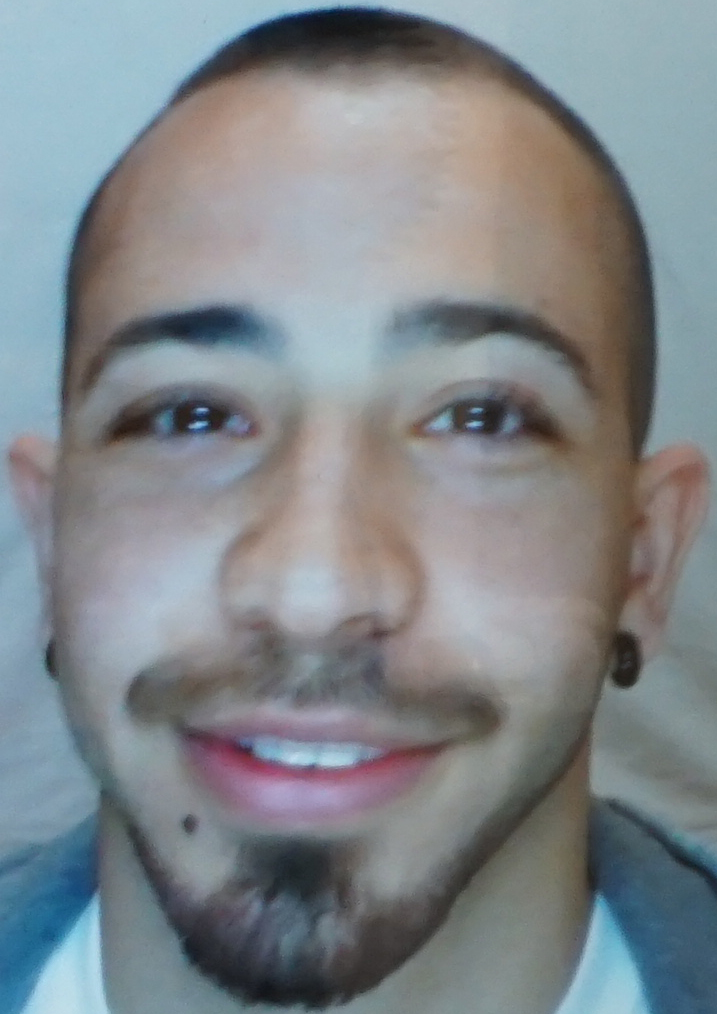
\includegraphics[width=0.18\textwidth]{images_databases/fravrgb/at4-1.JPG} \label{frav_im2-4}}
\subfigure[real user RGB]{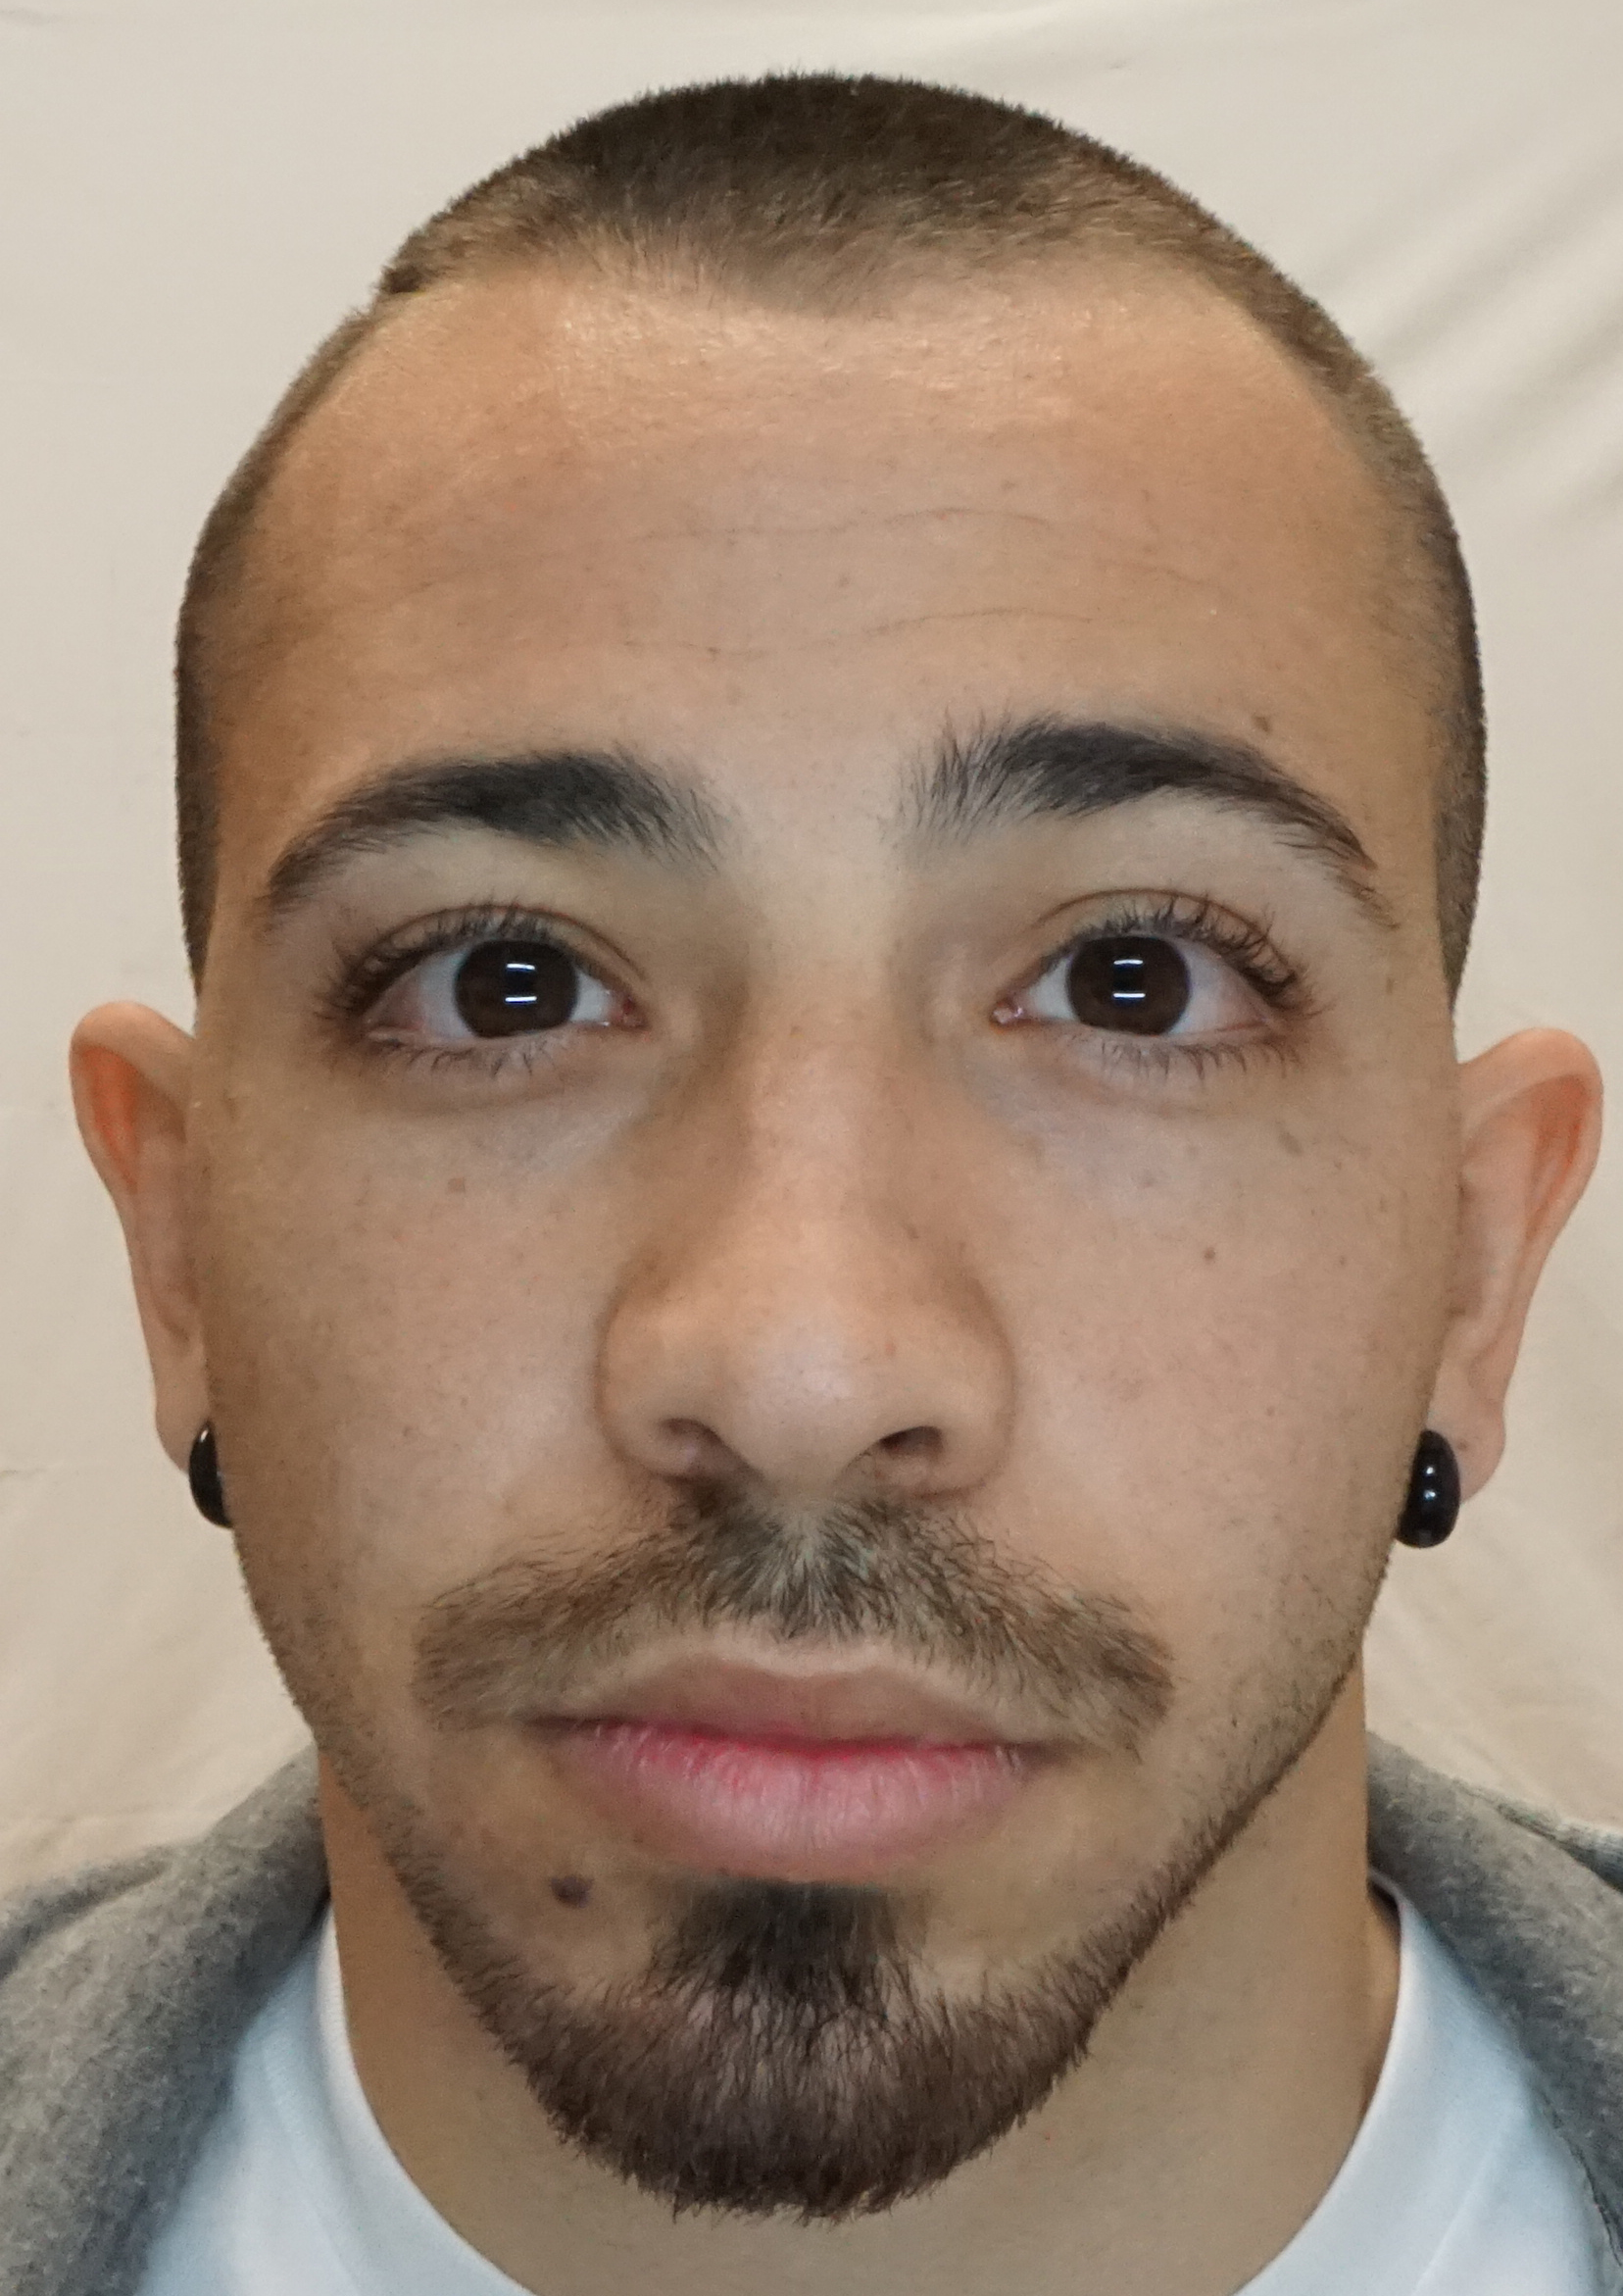
\includegraphics[width=0.18\textwidth]{images_databases/fravrgb/real1.JPG} \label{frav_im2-5}}

\subfigure[printed NIR image attack]{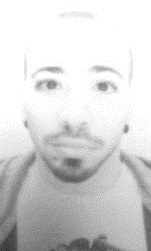
\includegraphics[width=0.18\textwidth]{images_databases/fravnnir/at-1.jpg} \label{frav_im3-1} }
\subfigure[mask attack NIR]{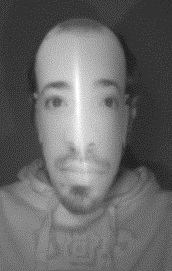
\includegraphics[width=0.18\textwidth]{images_databases/fravnnir/at-2.jpg} \label{frav_im3-2}}
\subfigure[eye mask attack NIR]{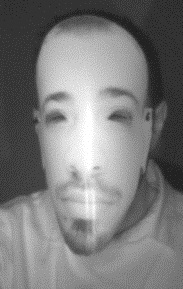
\includegraphics[width=0.18\textwidth]{images_databases/fravnnir/at-3.jpg} \label{frav_im3-3}}
\subfigure[tablet attack NIR]{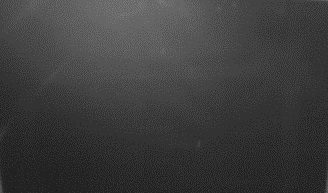
\includegraphics[width=0.18\textwidth]{images_databases/fravnnir/at-4.jpg} \label{frav_im3-4}}
\subfigure[real user NIR]{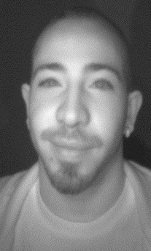
\includegraphics[width=0.18\textwidth]{images_databases/fravnnir/real.jpg} \label{frav_im3-5}}

\caption{Four attacks and real user of RGB and NIR FRAV database } \label{fig:RGB-frav2}
\end{figure}

When RGB and NIR (figure \ref{fig:RGB-frav2})images are used at the same time, two different methods, with the finality of using both types of images together, are determined:
\begin{itemize}
\item Adding images in characteristic level: adding the NIR image as another layer to RGB image, so the resultant image have hightxweightx4 dimensions (NIR images has one layer because it is a gray scale image and RGB images has three layers, one per each primary color). The network is feed with the resultant images like other times.
\item Adding images in classification level: after the network training and before feeding the classifier, RGB and NIR databases would be trained separately and its features would be appended as the input of the classifier.
\end{itemize}

To conclude, this database is going to be used in the three different ways: just RGB images, RGB and NIR images added in characteristic level or classification level.\\

When the classes are build, two ways are possible to be done: the first one where real people are one class (positive) and the different attacks are another class (negatives), so two classes have been used; and the second way where each attacks correspond with a class, so five classes (4 attacks and 1 real) have been utilized.\\

\subsection{CASIA dataset}
The CASIA Face Anti-Spoofing database is a database from the Chinese Academy of Sciences Centre for Biometrics and Security Research (CASIA-CBSR) \cite{Casiadatbase}.

CASIA database is formed by real or genuine images of people and three different attacks of the same people:
\begin{itemize}[itemsep=2pt,topsep=8pt,parsep=0pt,partopsep=20pt]
 \item Images of people printed (attack) represented in figure \ref{casia_im1-1}.
 \item Images of people with a mask with the eyes cropped (attack) represented in figure \ref{casia_im2-1}.
 \item Tablet attack represented in figure \ref{casia_im3-1}
\item Images of real users represented in figure \ref{casia_im4-1}.
 \end{itemize}

\begin{figure}[htb]
\centering
\subfigure[printed image attack]{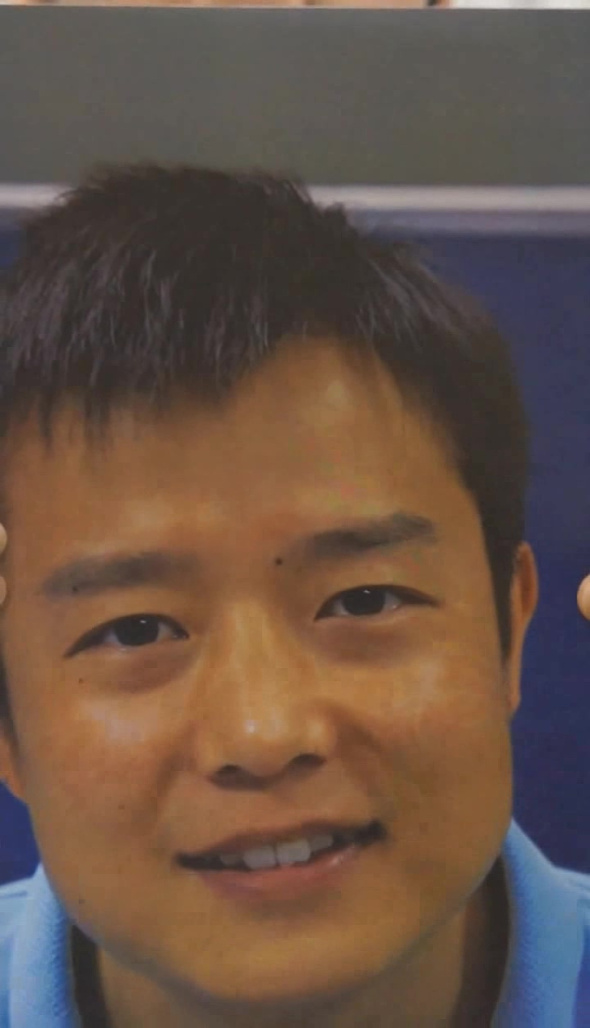
\includegraphics[width=0.2\textwidth]{images_databases/casia/at1-2.jpg} \label{casia_im1-1} }
\subfigure[eye printed image attack]{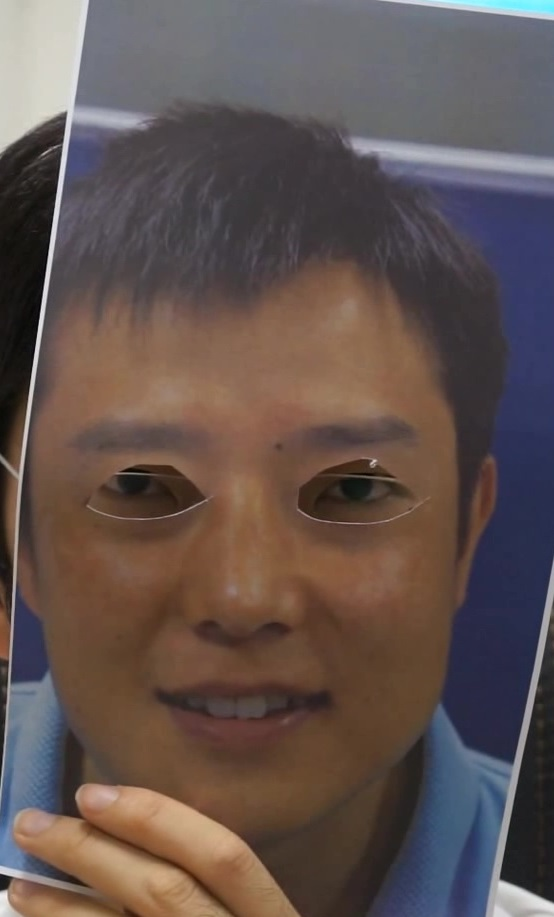
\includegraphics[width=0.2\textwidth]{images_databases/casia/at2-2.jpg} \label{casia_im2-1} }
\subfigure[tablet attack]{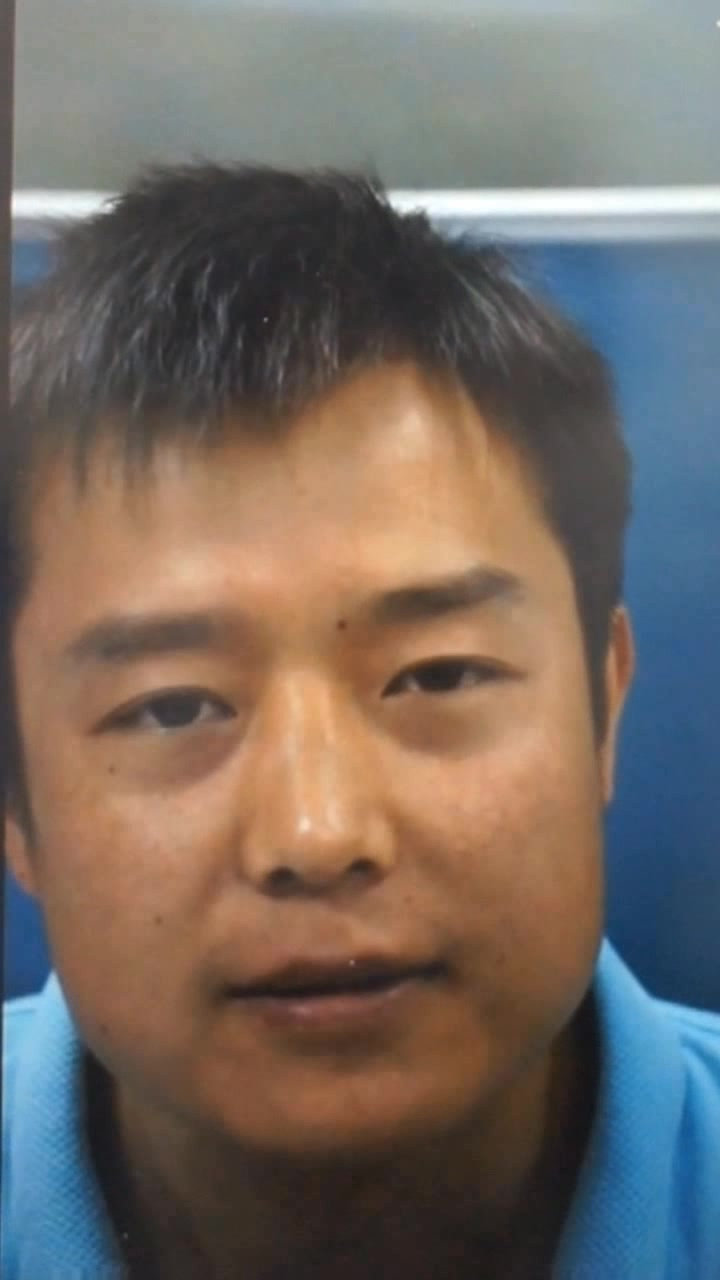
\includegraphics[width=0.2\textwidth]{images_databases/casia/at3-2.jpg} \label{casia_im3-1} }
\subfigure[real user]{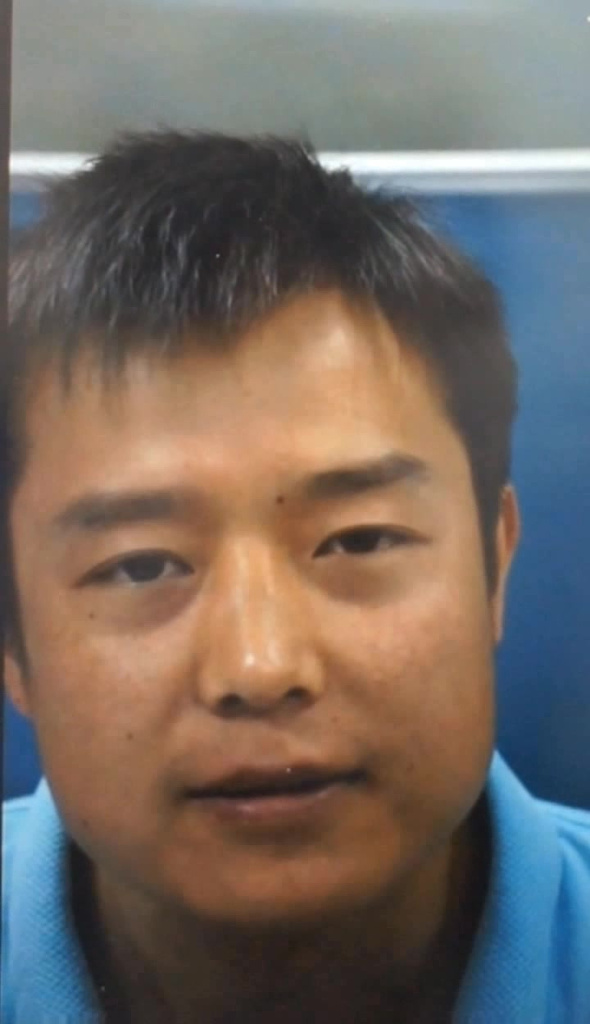
\includegraphics[width=0.2\textwidth]{images_databases/casia/real2.jpg} \label{casia_im4-1} }

\caption{Three attacks and real user from casia database } \label{fig:casia2}
\end{figure}

Originally, this database is a video database, in which each sample is a different video, but for the experiments developed no videos (entirely or fed directly to the network) have been used. The CASIA database has been used in two different ways:
\begin{itemize} [itemsep=2pt,topsep=8pt,parsep=0pt,partopsep=20pt]
 \item Using a single image per person and class. When this database is used, it is going to be referred as CASIA image database.
 \item Reading three frames per video and saving each frame as a independent image sample. This database is going to be referred as CASIA video database.
\end{itemize}

The characteristics of the CASIA image database are the following ones:
\begin{itemize}[itemsep=2pt,topsep=8pt,parsep=0pt,partopsep=20pt]
\item There are 49 images per user, so there are 196 unique samples.
\item Samples do not have the same size.
\item Samples are in RGB space.
\item The face of the image is centered.
\end{itemize}

The characteristics of the CASIA video database are the following ones:
\begin{itemize}[itemsep=2pt,topsep=8pt,parsep=0pt,partopsep=20pt]
\item There are 8 videos per person (two videos for real user, and two per each attack).
\item There are two videos because one is filmed horizontally and the other vertically, one filmed with a smartphone and the other with the frontal camera of a laptop.
\item There are 50 different users, so there are 400 different videos.
\item For each video 3 frames are read, so there are 1200 unique samples.
\item Samples are in RGB space.
\item Faces are centered in the image and blink expression and movement of people are produced.
\end{itemize}

At the time of assigning a class, it could be done using two classes, the positive class to the real users and the negative class to the attacks; If each attack is assigned to a independent class, it would be four different classes, the real user class and three attack classes.\\

%\begin{figure}[htb]
%\centering
%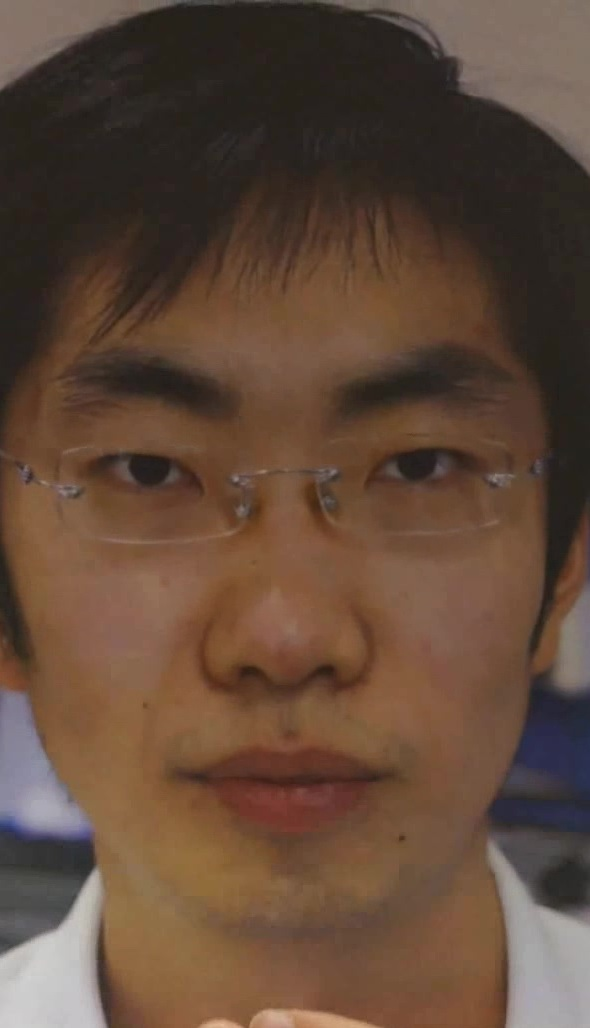
\includegraphics[width=0.2\textwidth]{images_databases/casia/at1-1.jpg}
%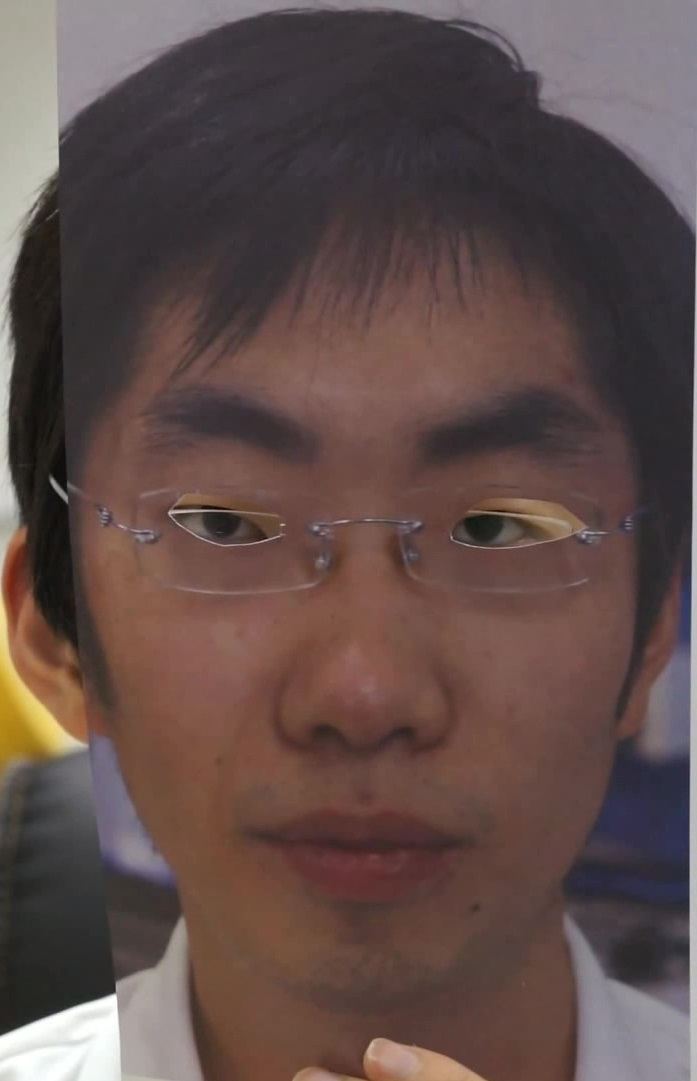
\includegraphics[width=0.2\textwidth]{images_databases/casia/at2-1.jpg}
%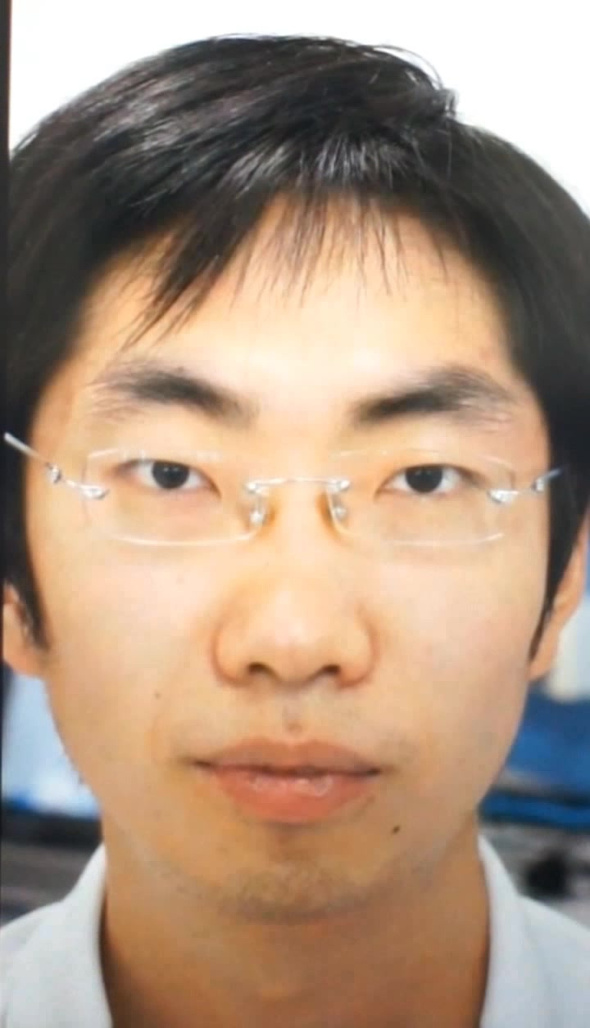
\includegraphics[width=0.2\textwidth]{images_databases/casia/at3-1.jpg}
%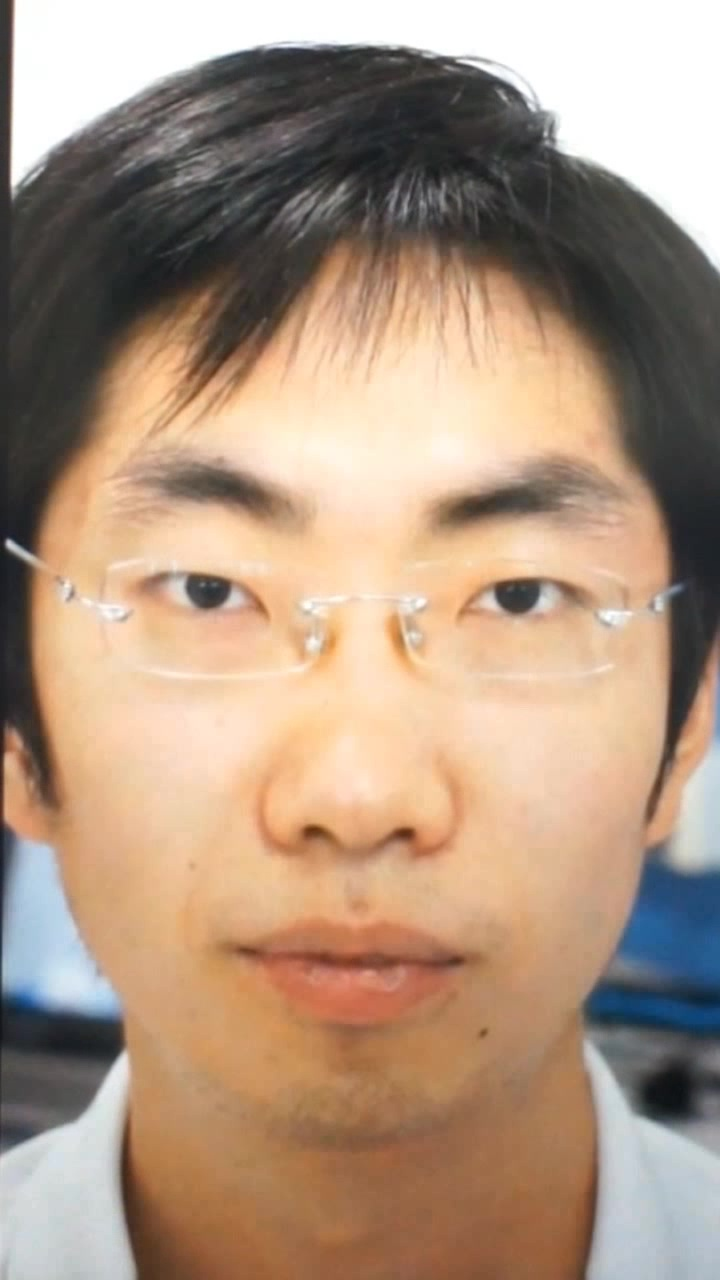
\includegraphics[width=0.2\textwidth]{images_databases/casia/real1.jpg}

%\caption{Three attacks and real user from casia database } \label{fig:casia1}
%\end{figure}

This database has been used in different articles \cite{yangLL14,Spoofing_survey,MSUdatabse,LSTM-CNN}, it is a very utilized databased for face biometrics.\\

\subsection{MSU-MFSD database}
The MSU Mobile Face Spoofing Database (MSU-MFSD) is a video face anti-spoofing database \cite{MSUdatabse}.\\

In figure \ref{fig:mfsd} are represented the three attacks and a real user which forms this database:
\begin{itemize}[itemsep=2pt,topsep=8pt,parsep=0pt,partopsep=20pt]
\item Printed photo attack represented in figure \ref{mfsd_im1-1}.
\item Tablet (iPad Air) attack where a video is Replayed represented in figure \ref{mfsd_im1-1}.
\item Smartphone (iPhone 5s) attack represented in figure \ref{mfsd_im1-1}.
\item Real user represented in figure \ref{mfsd_im1-1}.
\end{itemize}

\begin{figure}[htb]
\centering
\subfigure[printed image attack]{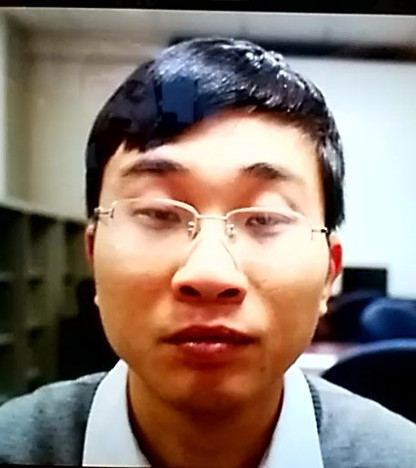
\includegraphics[width=0.2\textwidth]{images_databases/MFSD/at1-1.jpg} \label{mfsd_im1-1} }
\subfigure[tablet attack]{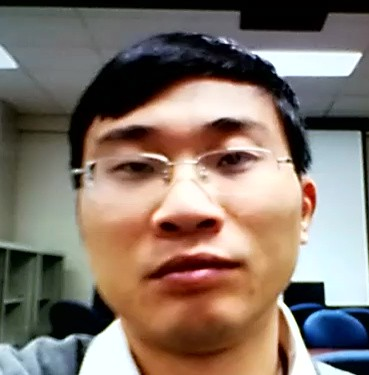
\includegraphics[width=0.2\textwidth]{images_databases/MFSD/at2-1.jpg} \label{mfsd_im2-1} }
\subfigure[smartphone attack]{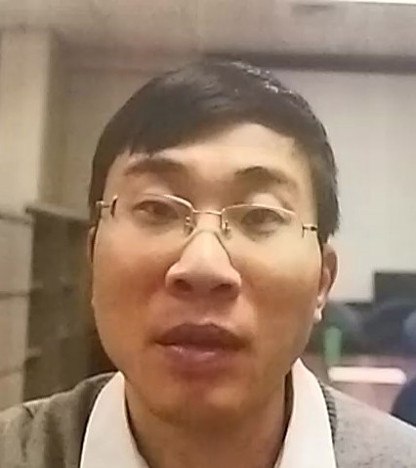
\includegraphics[width=0.2\textwidth]{images_databases/MFSD/at3-1.jpg} \label{mfsd_im3-1} }
\subfigure[real user]{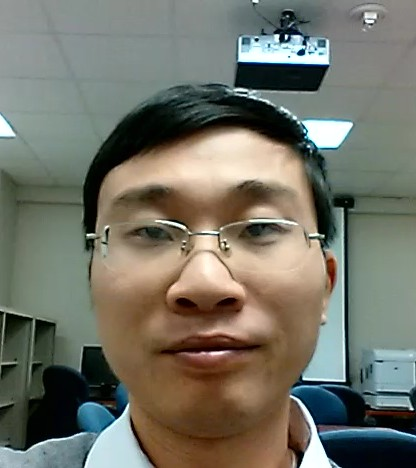
\includegraphics[width=0.2\textwidth]{images_databases/MFSD/1.jpg} \label{mfsd_im4-1} }

\caption{Three attacks and  real user from a person of MFSD database } \label{fig:mfsd}
\end{figure}

Originally, the database is a video database, but only one frame per user and class is used. The characteristics of the database are the following ones:
\begin{itemize}[itemsep=2pt,topsep=8pt,parsep=0pt,partopsep=20pt]
\item There are 35 images per attack or genuine user. There are 140 unique samples.
\item Images are in RGB space.
\item Faces are centred in images.
\item The size of each image are not equal. Approximately images are 300 pixel heigh and 335 pixel width.
\item Images have been acquired with a Macbook Air laptop and a Google Nexus4 smartphone.
\end{itemize}

%\begin{figure}[htb]
%\centering
%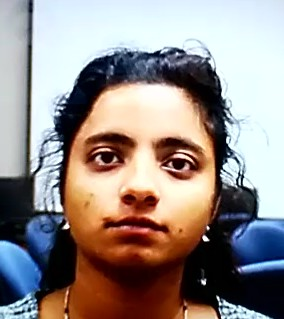
\includegraphics[width=0.2\textwidth]{images_databases/MFSD/at1-2.jpg}
%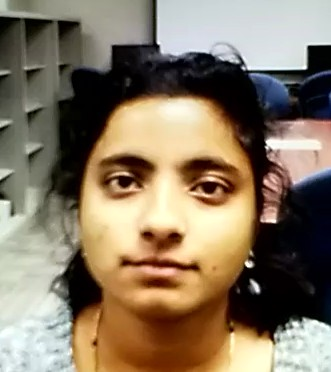
\includegraphics[width=0.2\textwidth]{images_databases/MFSD/at2-2.jpg}
%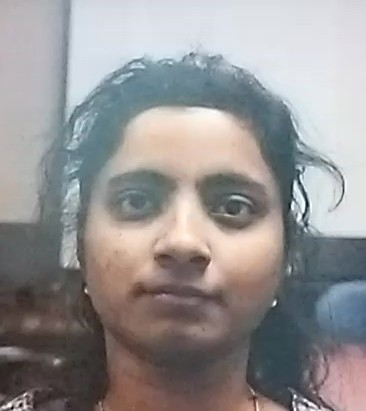
\includegraphics[width=0.2\textwidth]{images_databases/MFSD/at3-2.jpg}
%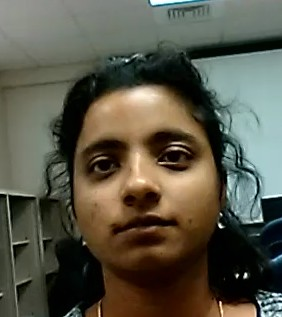
\includegraphics[width=0.2\textwidth]{images_databases/MFSD/2.jpg}
%\caption{Three attacks and real user from a user of MFSD database } \label{fig:mfsd2}
%\end{figure}

\section{Classifiers, Reduction of the dimensionality algorithms and Cross Validation}
Classifying is called to the task of assign a category to an object. The classification task is based in the obtained features of the object and the characteristics of the feature extractor \cite{Duda}. The particular case of this thesis, features obtained at the output of a Convolutional Neural Network are utilized for classification.\\

The output of the convolutional neural network could be bigger enough and some features could not be relevant for the classification. To solve the speed and robustness issues that could appear because of the quantity of features \cite{PCAvsLDA}, techniques to reduce the dimensionality are used.\\

Classifiers must be customized to each problem, to find the optimal parameters for each occasion, cross validation technique has been used.\\

\subsection{Classifiers}
In this section, the classifiers used along the thesis are described.\\

\subsubsection{Logistic Regression}
Logistic regression is a probabilistic and a linear classifier. It is customized by a weight matrix \textit{W} and a bias vector \textit{b}.\\

The logistic regression weights and bias define a linear hyperplane which is the decision boundary of the classes. In order to find the parameters, the Maximum likelihood estimation is used during training \cite{ClassifiersReview}:\\

\begin{equation}
\prod_{i=1}^{n}P(y_i|X_i,W,b)
\end{equation}

Given an input vector \textit{x}, which belongs to the \textit{i} class (a value of a stochastic variable \textit{Y}), its probability could be described as follows:

\begin{equation}
P(Y=i|x,W,b) = \frac{e^{W_ix+b_i}}{\sum_j e^{W_ix+b_i}}
\end{equation}

The class of a new sample ($y\_{pred}$) would be classified as:

\begin{equation}
y_{pred} = argmax_{i}P(y_i|X_i,W,b)
\end{equation}

A sample would belong to a class depending on position in the space with respect to the hyperplane that separates the classes.\\

\subsubsection{Support Vector Machine}
Support Vector Machine (SVM) is a two-class (bi-class) classifier. The smallest generalization error is linked to the \textit{margin} concept. Margin is the perpendicular distance between the closest sample of the database and the calculate hyperplane \cite{MachineLearning}. An hyperplane is optimal if the margin is the maximum and this margin is calculated (as the same way as logistic regression):\\

\begin{equation}
\underset{w b}{\operatorname{arg\,max}}\left \{ \frac{1}{||W||} \underset{n}{\operatorname{min}}[t_{n}(W^T \phi (X_n)+b)]   \right \}
\end{equation}


Where \textit{w, b} are the parameters that should be optimized in order to maximize the distance. \textit{$t_n$} are the training samples. $\phi$ is a fixed feature-space transformation, \textit{b} is the bias parameter.\\

\begin{figure}[htb]
\centering
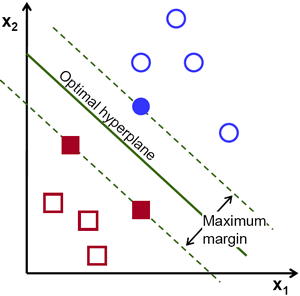
\includegraphics[width=0.5\textwidth]{images_miscelaneus/svm.png}
\caption{Optimal hyperplane and the decision boundary. Image obtained from \cite{SVMimage}.} \label{fig:SVM}
\end{figure}

In figure \ref{fig:SVM} the optimal hyperplane between two classes are represented with its corresponding margin. In the given example, the two classes are well differentiated. Figure \ref{fig:SVM} has been obtained from \cite{SVMimage}.\\

Based on estimate the hyperplane that maximize the distance between classes, the closest vectors of each class are selected \cite{SVM1, MachineLearning}. In practice, the margin is determined by \textit{C}, a parameter that should be chosen by user to get the optimal margin.\\

The SVM performance is join to a kernel function which allows variability in nonlinearity and flexibility in the model \cite{ClassifiersReview, practicalguideSVM}. There are various kernels (polynomial, sigmoid, etc.), two of them are utilized:

\begin{enumerate}
\item Linear kernel: $ K(x_{i},x_{j}) = x_i^T x_j$.
\item Radial basis function (RBF) kernel: $K(x_{i},x_{j}) = exp(-\gamma||x_i-x_j||^2), \gamma>0$
\end{enumerate}

\subsubsection{K Nearest Neighbours}
K- Nearest Neighbour (KNN) is a generative and non parametric classifier. For classifying, the density estimation procedure is utilized. The difference between this classifier and others is that data is used in this algorithm directly for classification, without building a model first \cite{ClassifiersReview}. The density function is determined by the form \cite{MachineLearning}:
\begin{equation}
p(x) = \frac{K}{N V}
\end{equation}

Where \textit{K} is the number of points inside the region \textit{R} whose volume is \textit{V} and \textit{N} is the number of total samples or observations.\\

This classifier uses the observation directly to classify and needs all the samples to predict a new one. The probability of a sample \textit{x} belonging to a class \textit{$C_k$} is defined by \cite{MachineLearning}:
\begin{equation}
p(x|C_k) = \frac{K_k}{N_k V}
\end{equation}

Where $N_k$ are the observations of a class $C_k$ and $K_k$ of it class points are contained in the volume \textit{V}.\\

The \textit{K} value is fixed and constant, it should be calculated and optimized by user of each application.\\

\subsubsection{Decision Tree}
Decision Tree classifier is based in a natural classification based in a sequence of true/false or yes/no questions \cite{Duda}. It could be used as a binary classifier or a \textit{k} classes classifier. \\

The input data is split to maximize its separation, resulting a tree structure \cite{ClassifiersReview} as is described in figure \ref{fig:Tree} (image obtained from \cite{Treeimage}). Where depending on the features, a sample changes from a principal branch to a branch of this until a class is signed. The last branches correspond to the classes and the same class could be in different final branches. \\

\begin{figure}[htb]
\centering
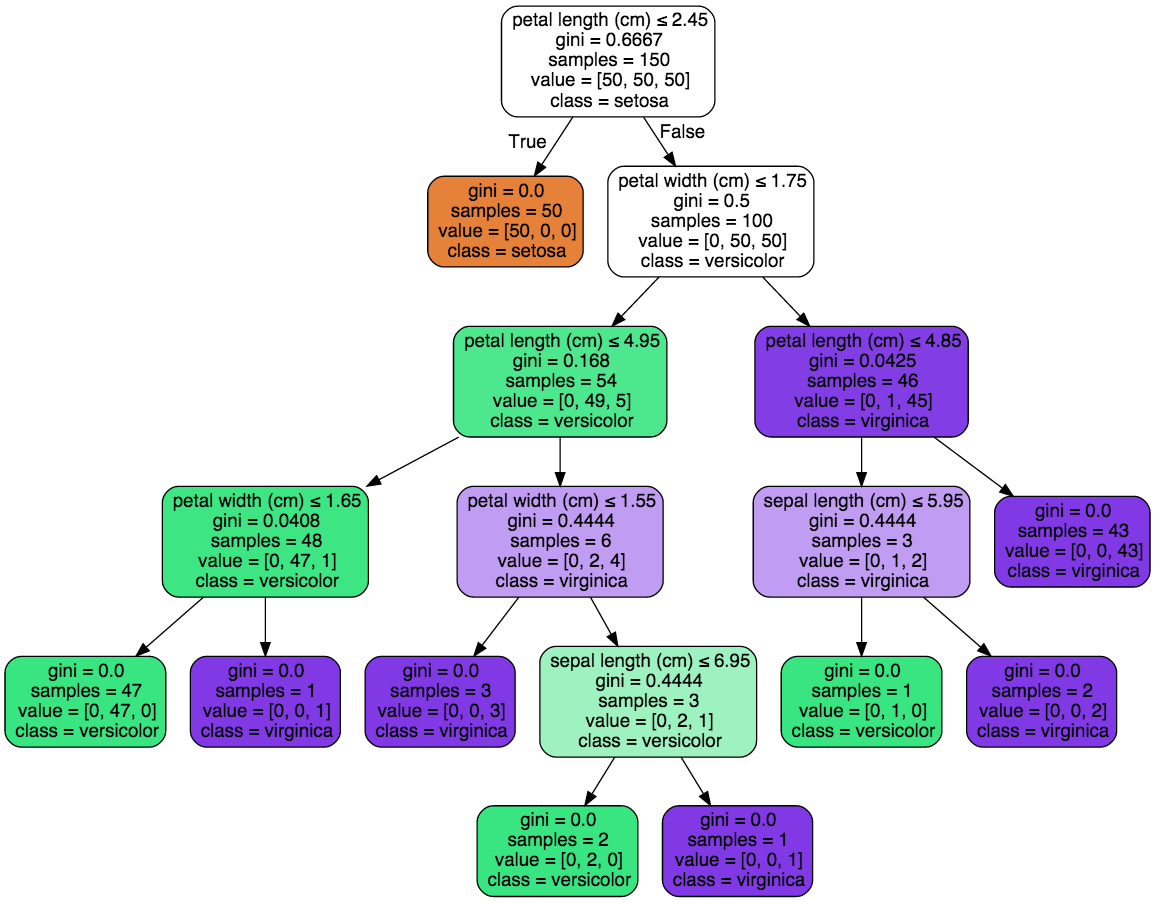
\includegraphics[width=0.55\textwidth]{images_miscelaneus/tree.png}
\caption{Decision Tree Classifier. Image obtained from \cite{Treeimage}.} \label{fig:Tree}
\end{figure}

\subsection{Dimensionality reduction algorithms}
The objective of those algorithms is transformed by the characteristic vector into another characteristic vector but with a lower dimensionality. Linear methods, that projects the dimensional data onto another space whose dimensionality is lower \cite{Duda}, have been used. The two techniques, the most common used, are described and used along the thesis.\\

\subsubsection{Linear Discriminant Analysis}
Linear Discriminant Analysis (LDA) looks for the vectors in the space that best discriminate among classes; LDA pretends to maximize the between-class measure (equation \ref{eq:Sb}) at the same time as the within-class measure (equation \ref{eq:Sw}) is minimized \cite{PCAvsLDA}.\\

\begin{equation}
S_w = \sum^c_{j=1}(\mu _j - \mu)(\mu _j - \mu)^T
\end{equation}\label{eq:Sb}

\begin{equation}
S_w = \sum^c_{j=1}\sum^{N_j}_{i=1}(X_i^j - \mu _j)(X_i^j - \mu _j)^T
\end{equation}\label{eq:Sw}

The data of \textit{d} dimensions would be projected onto a \textit{s} dimensions and being $s < d$. The minimum value that \textit{s} could take would depend on the number of classes \textit{n}: $s \geq n-1$.


\subsubsection{Principal Component Analysis}
Principal Component Analysis (PCA) uses a subspace \textit{t} in which the the variance direction among basis vectors is maximum in the original space \textit{f} \cite{PCAvsLDA}. PCA faces the problem of reducing the \textit{n} dimensional samples vector to a single vector $X_0$. The $X_0$ vector would be the smallest result of the sum of the squared distances between $X_0$ and various features $X_k$ \cite{Duda}.\\

The new subspace is usually smaller than the original space \cite{PCAvsLDA}.\\

The linear transformation from one space into another would be denoted as \textit{W}, and its columns are eigenvalues which has eigenvectors associated.\\

The feature vectors (\textit{y}) from the \textit{f} space would depend on \textit{W}:

\begin{equation}
y_{i} = W^TX_{i}, i=1,...,N
\end{equation}

Being \textit{N} the total number of feature vectors.\\

\subsection{Cross Validation}
Classifiers are defined by certain parameters. For example,the number of neighbours (\textit{k}) in KNN classifier is a value that user have to determine. In this case is useful use Cross Validation to determine the value of \textit{k}.\\

This method uses the training samples. They are split in groups (\textit{kfolds}) and used to train and test the classifier with different values; in the KNN case, the value k would be change. A metric (score) is calculated and it is possible to determine the value of the classifier in which the metric is the optimum.\\

This technique has been usedto calculate the value which a classifier is defined. For SVM classifier the value \textit{C}, for KNN classifier the value {k}, for Decision Tree classifier the depth of the tree, softmax classifier to determine the learning rate when it has not been trained at the same time of the network and for PCA and LDA the number of components. \\

%!TEX root = Memoria_TFM.tex
\section{Metrics}
To characterize a system, it is necessary metrics that evaluate it. In this section the used metrics along the thesis are exposed.\\

Before describing the parameters it is necessary define that the posed problem is bi-class, that means that only two classes would be used:

\begin{description}
\item \textbf{Positive class}: are the samples of the real users, the genuine or \textit{bona fide}.
\item \textbf{Negative class}: are the different attacks samples which that pretend to be real users but not.
\end{description}

\subsection{Cost and Error rate}
The first parameter that is used is the cost. The cost is used while the neural network is training, in fact, is the value that must be minimized during the training. The lower value, The better performance of the network.\\

The cost calculated with the Minibatch Stochastic Gradient Descent (MSGD) is the Negative Log-Likelihood Loss. The MSGD is a variant of the Stochastic Gradient Descent in which the cost is calculated with a mini batch of data, not each sample independently and the Loss is the accumulation \cite{Stutz}.\\

The loss is calculated in the following way:\\

\begin{equation}
  Loss(\theta, D) = - \sum_{i=0}^{|D|}log P(Y = y^{(i)}|x^{(i)}, \theta)
\end{equation}

The error in the validation process is calculated after the logistic regression classification, because is the classifier used during the training process. The error during the testing procedure depends on the used classifier. In both cases, the error represents the number of misclassified samples over the total samples used.\\

\subsection{True Positives (TP), True Negatives (TN), False Positives (FP), False Negatives (FN)}
If each predicted class is compared with it real target, True Positives (TP), True Negatives (TN), False Positives (FP), False Negatives (FN) values could be calculated. These metrics are usually used for bi-classes problems.\\

Those metrics, are gotten when positive or negative samples are correctly or incorrectly classified \cite{Sokolova}. The classified or predicted sample is compared with its real target.\\

If a positive sample is classified as positive is a true positive (TP), but if it has been classified as negative is a false negative (FN).\\

If a negative sample is classified as negative is a true negative (TN), but if it has been classified as positive, is a false positive (FP).\\

From those four metrics, it could be extracted the confusion matrix for binary classification which is defined in table \ref{table:ConfusionMatrix} \cite{ROC, Sokolova}:

\begin{table}[htb]
\centering
\begin{tabular}{|
>{\columncolor[HTML]{ECF4FF}}c |>{\columncolor[HTML]{FFFFFF}}c | >{\columncolor[HTML]{FFFFFF}}c |}
\hline
\textbf{Real / Classified} & \cellcolor[HTML]{ECF4FF}\textbf{Positive} & \cellcolor[HTML]{ECF4FF}\textbf{Negative} \\ \hline
\textbf{Positve}           & TP                                        & FN                                        \\ \hline
\textbf{Negative}          & FP                                        & TN                                        \\ \hline
\end{tabular}
\caption{Confusion Matrix.} \label{table:ConfusionMatrix}
\end{table}

The confusion Matrix resume these four metrics in a table. Both, the confusion matrix or the parameters individually, are widely utilized.\\

\subsection{ROC curve and Equal Error Rate (EER)}
From the confusion matrix, it is possible calculate others parameters \cite{Sokolova}: precision, recall, specificity, accuracy, etc. because its values depend on TP, TN, FP, FN:\\

\begin{itemize}
\item The False Positive Rate (FPR) is defined as the proportion of all the negative samples (\textit{N}) that are classified as positive incorrectly \cite{ROC}:

\begin{equation}
FPR = \frac{FP}{N}
\end{equation}
Where:
 \begin{equation}
  N = FP + TN
\end{equation}

\item The True Positive Rate (TPR) is defined as the proportion of all the positive samples (\textit{P}) that are classified correctly \cite{ROC}. This parameter could be known as Recall too:
\begin{equation}
TPR = Recall = \frac{TP}{P}
\end{equation}
Where:
 \begin{equation}
  P = TP + FN
\end{equation}
%TPR could be called sensitivity and FPR could be calculated as 1 – specificity \\
\item False Acceptance Rate (FAR): is defined as the incorrectly accepted users with respect all the samples.
\begin{equation}
  FAR = \frac{FP}{P + N}
\end{equation}

\item False Rejection Rate (FRR): is defined as the incorrectly rejected users with respect all the samples.
\begin{equation}
  FRR = \frac{FN}{P + N}
\end{equation}

%\item Precision is defined as the proportion of real positive samples that has been classified as positive \cite{ROC,Sokolova}:
%\begin{equation}
 % precision = \frac{TP}{TP + FP}
%\end{equation}

\item Accuracy is defined as the proportion of the correctly classified samples of all the samples \cite{Sokolova}. The classifiers implemented in scikit-learn library return this value as metric.:
\begin{equation}
  Accuracy = \frac{TP + TN}{TP + FP + FN + TN}
\end{equation}
\end{itemize}

The Receiver Operator Characteristic (ROC) curve is the representation how the number of positives samples, which has been classified correctly, changes with the number of negative samples incorrectly classified. The ROC curve is defined by the parameters False Positive Rate (FPR) and True Positive Rate (TPR) \cite{ROC}.\\

\begin{figure}[htb]
  \centering
  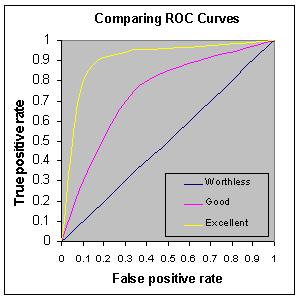
\includegraphics[width=0.4\textwidth]{images_miscelaneus/roccomp.jpg}
  \caption{ROC curves. Image obtained from \cite{RocImage}.}
  \label{RocImage}
\end{figure}

The figure \ref{RocImage}, obtained from \cite{RocImage}, demonstrates a ROC graph in which three curves are portrayed.  The yellow one represents a good classification, it is the desired ROC curve, but the blue curve represents a bad classification and it is not the desired result.\\

From the ROC curve, the Area Under the Curve (AUC) could be obtained, this value is the integral of the ROC curve, and its maximum value is 1 that means a perfect performance of the classifier. If the value of this parameter is lower than 0.7 the classifier performance required to be improved significantly.\\

From FAR and FRR rates it is possible to calculate the Equal Error Rate (ERR) and it is obtained at the point where FAR and FRR acquire the same value. The closest is its value to 0, the better is the performance of the classifier.\\
%The Precision and Recall curve is the representation of the Precision and the Recall in the same graph. The desired behaviour of a classification system is a high recall (1) and a high precision (1) because that would mean that predictions made by the classifier are correct.\\

\subsection{APCER and BPCER}
The ISO/IEC 30107-3 \cite{ISO} is the collaboration result of  the International Organization for Standardization (ISO) with the International Electrotechnical Commission (IEC).\\

The ISO defines the terms related to the tests, the reports and the biometric presentation of biometrics systems. In addition, the performance methods, specify principles as well as metrics are defined. From this document, the APCER, BPCER and APCER-BPCER curve metrics have been obtained:\\

Attack Presentation Classification Error Rate (APCER) is defined as the proportion of presentation attacks that has been classified incorrectly (as \textit{bona fide} presentation.)\\

\begin{equation}
  APCER_{PAIS} = \frac{1}{N_{PAIS}}\sum_{i=1}^{N_{PAIS}}(1 - Res_{i})
\end{equation}

\textit{Bona fide} Presentation Classification Error Rate (BPCER) is defined as the proportion of \textit{bona fide} presentations  incorrectly classified as presentation attacks.\\

\begin{equation}
  BPCER = \frac{\sum_{i=1}^{N_{BF}}Res_{i}}{N_{BF}}
\end{equation}

where: \begin{itemize}
\item $N_{BF}$ is the number of \textit{bona fide} presentations
\item $Res_{i}$ is 1 if $i^{th}$ presentation is classified as an attack and 0 if is classified as a \textit{bona fie} presentation.
\item $N_{PAIS}$ is the number of attack presentations
\end{itemize}

The APCER-BPCER curve illustrates in the same graph both parameters. The ideal system would have a low APCER (0) and a low BPCER (0) because it means that samples are not incorrectly classified.\\

\section{Algorithm diagram chart}
The flowchart of the code used for this thesis development in section \ref{sec:adapt_lenet} is shown in \ref{fig:flowchart}. In the figure, the subsets generation flowchart from the databases is presented in \ref{fig:dat_flowchart}; it has been used for each database (CASIA images, CASIA videos, RGB FRAV, RGB+NIR feature level FRAV, RGB+NIR classification level FRAV and MFSD-MSU). The programmed code is summarized in figure \ref{fig:alg_flowchart} which has been run, as described in the figure, as many times as databases are available.


\begin{figure}[tb]
\centering
\subfigure[Subsets generator diagram]{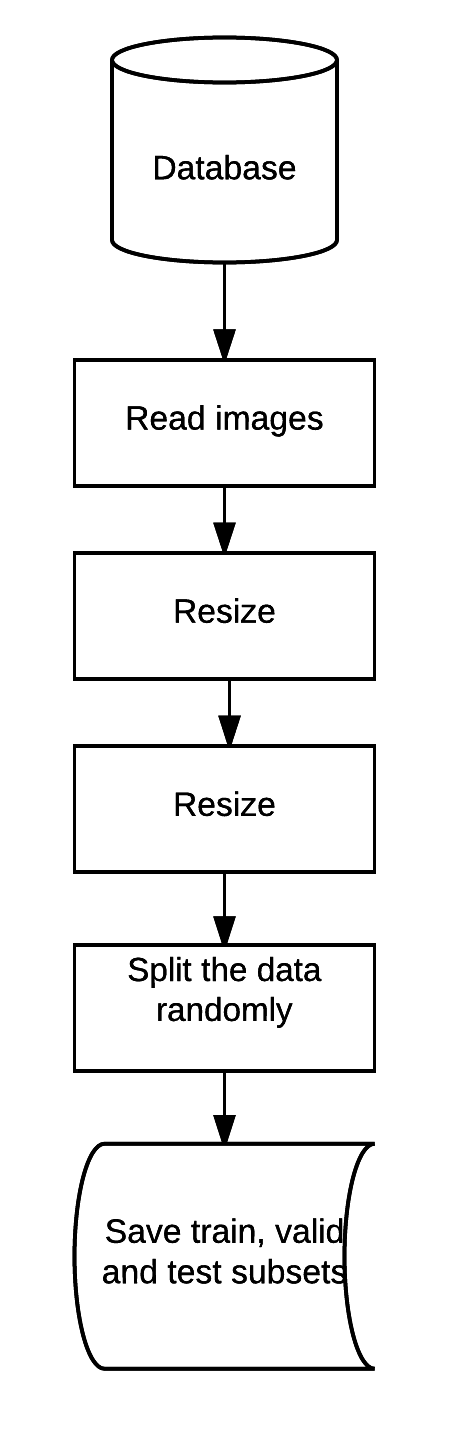
\includegraphics[width=0.18\textwidth]{images_miscelaneus/Databases_gen.png}\label{fig:dat_flowchart} }
\subfigure[General algorithm diagram]{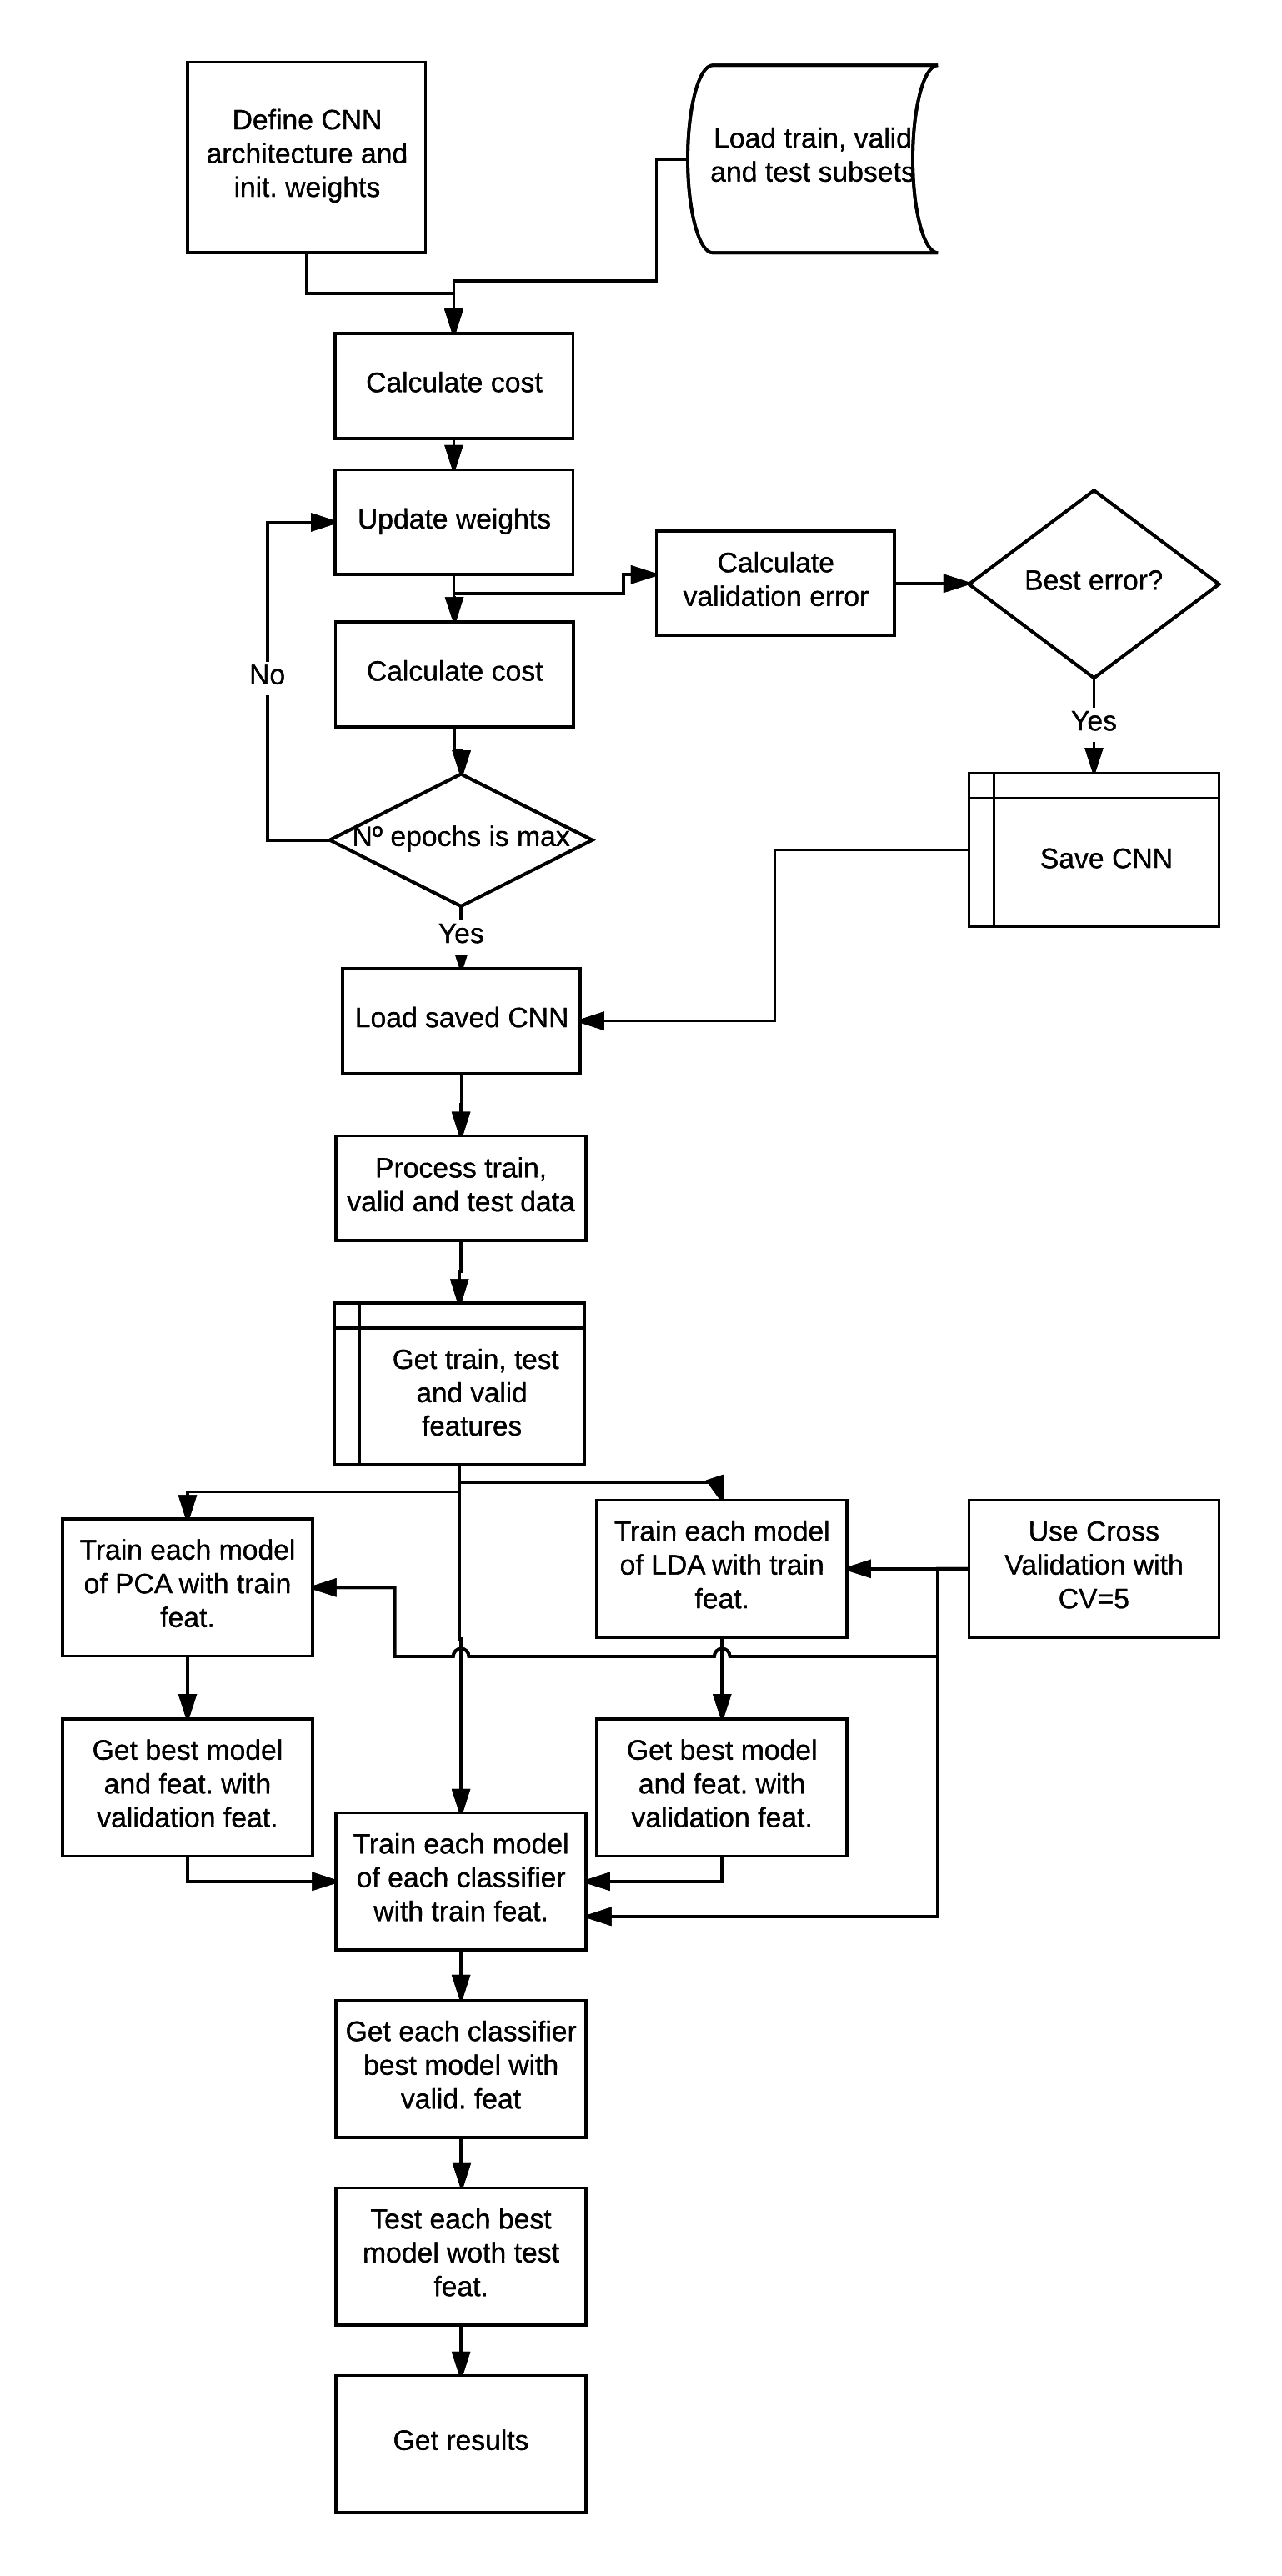
\includegraphics[width=0.62\textwidth]{images_miscelaneus/Algorithm.png} \label{fig:alg_flowchart} }
\caption{Code diagram chart.}
\label{fig:flowchart}
\end{figure}
